\documentclass[9pt,twocolumn,twoside]{pnas-new}
% Use the lineno option to display guide line numbers if required.
% Note that the use of elements such as single-column equations
% may affect the guide line number alignment. 

\templatetype{pnasresearcharticle} % Choose template 
% {pnasresearcharticle} = Template for a two-column research article
% {pnasmathematics} = Template for a one-column mathematics article
% {pnasinvited} = Template for a PNAS invited submission

% added to enable supplementary figures
\usepackage{placeins}
\usepackage{newfloat}
\DeclareFloatingEnvironment[name={Figure}]{suppfigure}
\renewcommand{\thesuppfigure}{S\arabic{suppfigure}}

\DeclareFloatingEnvironment[name={Dataset}]{suppdata}
\renewcommand{\thesuppdata}{S\arabic{suppdata}}

\newcommand{\comment}[1]{{\color{red}[\textsl{#1}]}}

\title{Deep mutational scanning of hemagglutinin helps distinguish the evolutionary fate of human H3N2 influenza virus lineages}

% Use letters for affiliations, numbers to show equal authorship (if applicable) and to indicate the corresponding author
\author[a,d,e,1]{Juhye M. Lee}
\author[b,f,1]{John Huddleston} 
\author[a,d,e]{Michael B. Doud}
\author[a,f]{Kathryn A. Hooper}
\author[b,c,2]{Trevor Bedford}
\author[a,c,d,2]{Jesse D. Bloom}

\affil[a]{Basic Sciences Division}
\affil[b]{Vaccine and Infectious Diseases Division}
\affil[c]{and Computational Biology Program, Fred Hutchinson Cancer Research Center, Seattle, WA 98109, USA}
\affil[d]{Department of Genome Sciences}
\affil[e]{Medical Scientist Training Program}
\affil[f]{and Molecular and Cellular Biology Program, University of Washington, Seattle, WA 98195, USA}

% Please give the surname of the lead author for the running footer
\leadauthor{Lee} 

% Please add here a significance statement to explain the relevance of your work
\significancestatement{Authors must submit a 120-word maximum statement about the significance of their research paper written at a level understandable to an undergraduate educated scientist outside their field of speciality. The primary goal of the Significance Statement is to explain the relevance of the work in broad context to a broad readership. The Significance Statement appears in the paper itself and is required for all research papers.}

% Please include corresponding author, author contribution and author declaration information
\authorcontributions{Please provide details of author contributions here.}
\authordeclaration{Please declare any conflict of interest here.}
\equalauthors{\textsuperscript{1}J.M.L. and J.H. contributed equally to this work.}
\correspondingauthor{\textsuperscript{2}To whom correspondence should be addressed: trevor@bedford.io, jbloom@fredhutch.org}

% Keywords are not mandatory, but authors are strongly encouraged to provide them. If provided, please include two to five keywords, separated by the pipe symbol, e.g:
\keywords{influenza virus $|$ hemagglutinin $|$ deep mutational scanning $|$ antigenic drift $|$ epistasis} 

\begin{abstract}
% no more than 250 words. (200 now)
The evolution of seasonal H3N2 influenza virus is mediated by the rapid accumulation of mutations. 
A better understanding of how mutations affect viral growth is critical for studying the pressures and constraints underlying the evolution of the influenza virus in nature. 
Here we experimentally measure the effect of every possible single amino-acid mutation to an H3 influenza hemagglutinin on viral growth in cell culture. 
We find the stalk domain to be fairly mutationally tolerant, and there is not a large disparity in tolerance between the head and stalk domains.
Furthermore, our measurements reveal mutations in successful seasonal influenza viral lineages to be significantly more preferred than mutations in lineages that have died out, and this was true at both epitope and non-epitope sites.
Epistasis in hemagglutinin is also seemingly driven by antigenic drift.
The preferences measured in a distantly related protein homolog do not reveal such differences in viral lineages.
A comparison of the preferences between the two hemagglutinin homologs suggests that mutational effects increasingly shift as proteins diverge.
Overall, our work highlights how experimental measurements of mutational effects can be leveraged to gain insight into the evolutionary fates of viral strains and potentially be used to predict viral evolution.
\end{abstract}

\dates{This manuscript was compiled on \today}
\doi{\url{www.pnas.org/cgi/doi/10.1073/pnas.XXXXXXXXXX}}

\begin{document}

% Optional adjustment to line up main text (after abstract) of first page with line numbers, when using both lineno and twocolumn options.
% You should only change this length when you've finalised the article contents.
\verticaladjustment{-2pt}

\maketitle
\thispagestyle{firststyle}
\ifthenelse{\boolean{shortarticle}}{\ifthenelse{\boolean{singlecolumn}}{\abscontentformatted}{\abscontent}}{}

% If your first paragraph (i.e. with the \dropcap) contains a list environment (quote, quotation, theorem, definition, enumerate, itemize...), the line after the list may have some extra indentation. If this is the case, add \parshape=0 to the end of the list environment.
\dropcap{S}easonal H3N2 influenza virus evolves rapidly, readily accumulating mutations in the hemagglutinin (HA) surface protein that contribute to antigenic drift.
The evolution of human H3N2 influenza virus is further characterized by strain competition and frequent population turnover~\cite{fitch1997long,strelkowa2012clonal,bedford2015global}, producing a distinct spindly shape in its phylogenetic tree with a persistent trunk lineage and short-lived side branches~\cite{fitch1991positive} (Figure~\ref{fig:H3N2_phylogeny}).
Given the rather distinctive pattern of H3N2 evolution and that vaccination remains an effective way of reducing disease burden, a key challenge in selecting a vaccine strain lies in being able to predict the dominant strain in the upcoming influenza season.

Vaccine strain selection decisions mainly rely on experimentally characterizing the antigenicity of circulating strains.
To aid in the timeliness and throughput of making such decisions, previous work have endeavored to accurately predict the evolutionary outcomes of viral strains based on the antigenicity and/or tree structure of viral clades~\cite{steinbruck2014computational,neher2014predicting}.
However, the accuracy of these predictions are subject to uneven geographical and temporal sampling, and for~\cite{neher2014predicting}, the lack of information about a mutation's effect on antigenicity.
Others have attempted to model the antigenic properties of viral strains using sequence information or phylogenetic relationships~\cite{sun2013using,harvey2016identification,neher2016prediction}.

While mutations that contribute to antigenic evolution of the virus certainly determine strain success, the non-antigenic impacts of mutations play an important role in determining the persistence of viral strains~\cite{pybus2007phylogenetic,kucharski2011influenza,strelkowa2012clonal,luksza2014predictive,koelle2015effects}.
Due to the high mutation rate of RNA viruses \comment{citation here} and because the influenza virus does not appreciably recombine within a given segment, deleterious mutations become linked to beneficial ones.
A predictive fitness model takes into account mutations at both antigenic and non-antigenic sites in HA to infer clade fitness~\cite{luksza2014predictive}.
In this model, mutations at epitope sites are beneficial to viral fitness, while mutations at non-epitope sites incur a fitness cost.
Although this assumption may generally be true, the effect of mutations on viral fitness, and particularly on protein function, are much more nuanced.
We therefore need a greater understanding of the phenotypic effects of mutations on viral growth to comprehend the forces and constraints shaping influenza virus evolution in nature.


\begin{figure}
\centering
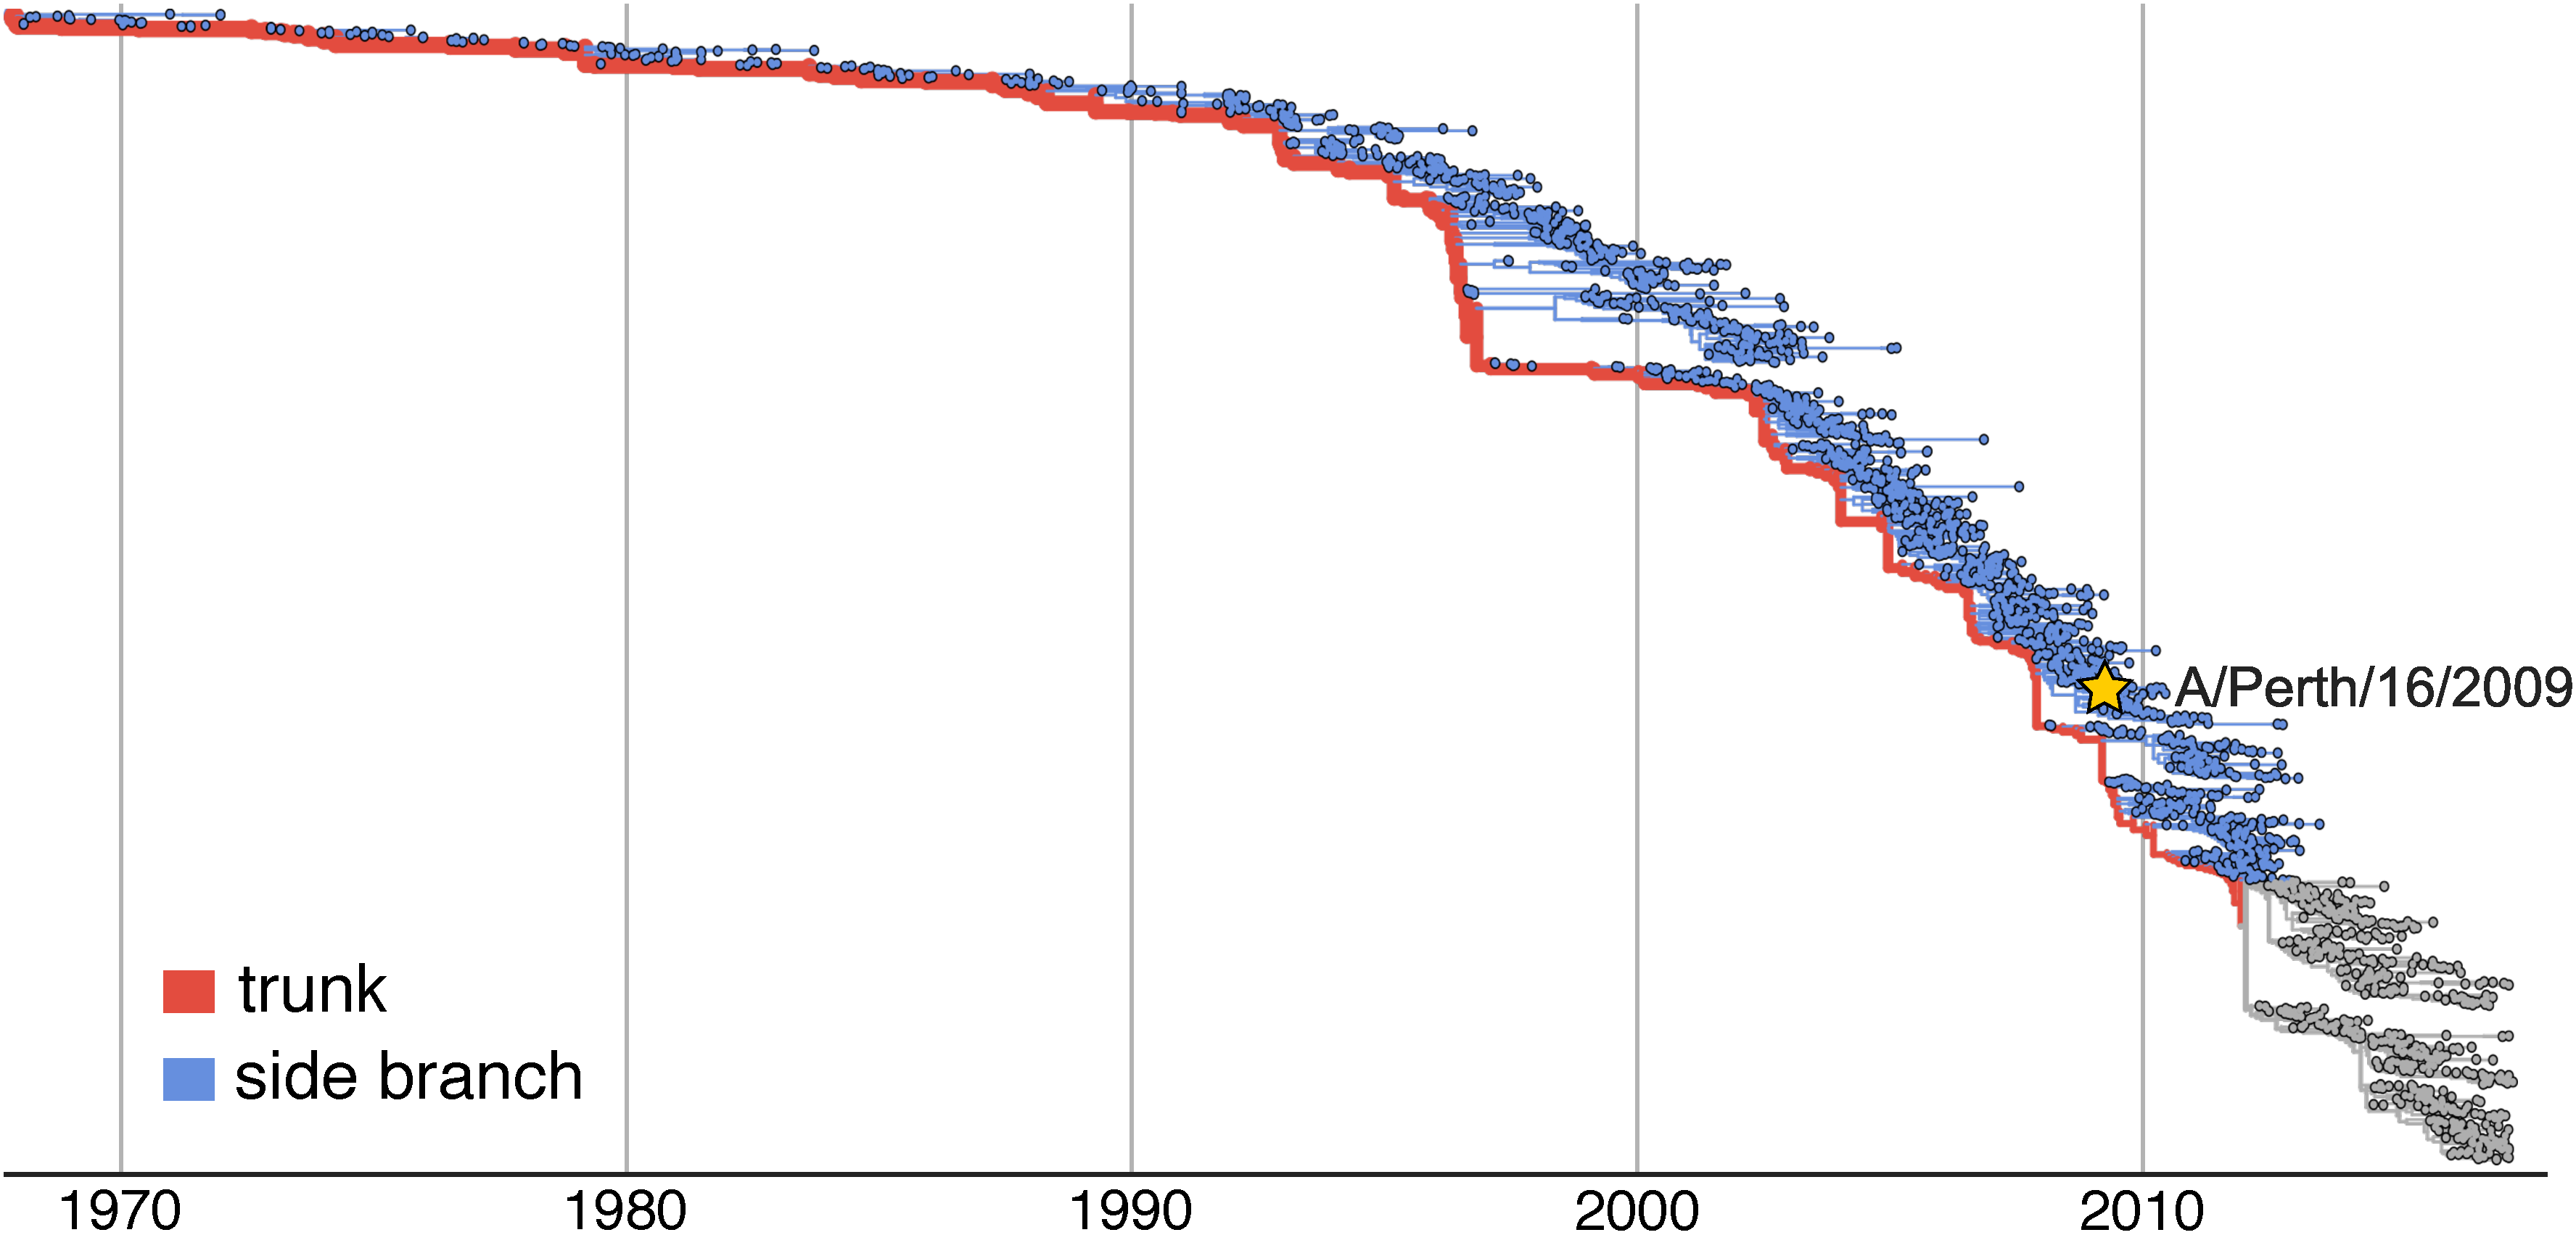
\includegraphics[width=\linewidth]{figs/H3N2_phylogeny/H3N2_phylogeny.pdf}
\caption{\label{fig:H3N2_phylogeny}
{\bf Human H3N2 HA phylogeny from 1968-2017.}
The trunk is shown in red, and side branches are shown in blue.
The gray branches represent the part of the tree for which we cannot yet distinguish the trunk from side branches.
The Perth/2009 strain is indicated with a star.
}
\end{figure}


We can measure such mutational effects in the lab using deep mutational scanning approaches~\cite{fowler2010high}.
Previously, we experimentally measured the effect of all possible single amino-acid mutations to an H1 HA from the A/WSN/1933 (H1N1) strain~\cite{thyagarajan2014inherent,doud2016accurate}.
However, the WSN/1933 is a highly lab-adapted strain, and these measurements may not be particularly relevant for studying the mutational processes of more contemporaneous strains circulating in the human population.
Here we measure the effects of mutations to the HA from the A/Perth/16/2009 (H3N2) strain on viral growth in cell culture.
% Our measurements generally agree with what is already known about HA structure and function.
We apply these experimental measurements to examine differences in the trunk and side branch lineages of human H3N2 influenza virus.
Trunk mutations were found to be more favorable than side branch mutations, both at epitope and non-epitope sites.
We also find evidence that epistasis in HA has primarily been driven by antigenic drift.
The measurements also enabled a comparison of how the amino-acid preferences have shifted between two diverged HAs.
The extent of shifts in amino-acid preferences increase as homologs diverge.
Our work highlights the potential for using high-throughput experimental measurements of mutational effects to inform evolutionary forecasting of human seasonal influenza virus.

\section*{Results}
\label{sec:results}

\subsection*{Deep mutational scanning of HA from a recent strain of human H3N2 influenza virus}
We performed a deep mutational scan to measure the effects of all amino-acid mutations to HA from the A/Perth/16/2009 (H3N2) strain on viral replication in cell culture. 
This strain was the H3N2 component of the influenza vaccine from 2010-2012~\cite{who2010d,who2011}.
Relative to the consensus sequence for this HA in Genbank, we used a variant with two mutations that enhanced viral replication in cell culture, G78D and T212I (Figure~\ref{suppfig:Perth2009_mut} and Dataset~\ref{suppdata:PerthHA}).
The G78D mutation occurs at low frequency in natural H3N2 sequences, and T212 is a site where a mutation to Ala rose to fixation in human influenza in $\sim$2011.

We mutagenized the entire HA coding sequence at the codon level to create mutant plasmid libraries harboring an average of $\sim$1.4 codon mutations per clone (Figure~\ref{suppfig:SangerSeq}).
We then generated mutant virus libraries from the mutant plasmids using a helper-virus system that enables the efficient generation of complex influenza virus libraries~\cite{doud2016accurate} (Figure~\ref{fig:dms_overview}A).
These mutant viruses derived all of their non-HA genes from the lab-adapted WSN/1933 strain.
Using WSN/1933 for the non-HA genes reduces biosafety concerns, and also helped increase viral titers.
To further increase viral titers, we used MDCK-SIAT1 cells that we had engineered to constitutively express the TMPRSS2 protease, which facilitates HA cleavage and activation~\cite{bottcher2006proteolytic, bottcher2010cleavage}.

After generating the mutant virus libraries, we passaged them at low MOI in cell culture to create a genotype-phenotype link and select for functional HA variants (Figure~\ref{fig:dms_overview}A).
All of the experiments were completed in full biological triplicate (Figure~\ref{fig:dms_overview}B). 
We also passaged and deep sequenced library 3 in duplicate (denoted as library 3-1 and 3-2) to gauge to the amount of experimental noise occurring \textit{within} a single biological replicate.
As a control to measure sequencing and mutational errors, we used the unmutated HA gene to generate and passage viruses carrying wildtype HA.

Deep sequencing of the initial plasmid mutant libraries and the passaged mutant viruses allowed us to observe selection for functional HA mutants.
As expected, selection against non-functional HA variants as led to reduced mutation frequencies in the mutant viruses compared to the initial mutant plasmids (Figure~\ref{fig:dms_overview}C).
Specifically, stop codons were purged to 20-45\% of their initial frequencies after correcting for error rates estimated by sequencing the wildtype controls.
The incomplete purging of stop codons is likely because genetic complementation due to co-infection~\cite{marshall2013influenza} enabled the persistence of some virions with nonfunctional HAs. 
We also observed selection against many nonsynonymous mutations, with their frequencies falling to 30-40\% of their initial values after error correction.

\begin{SCfigure*}[\sidecaptionrelwidth][t]
\centering
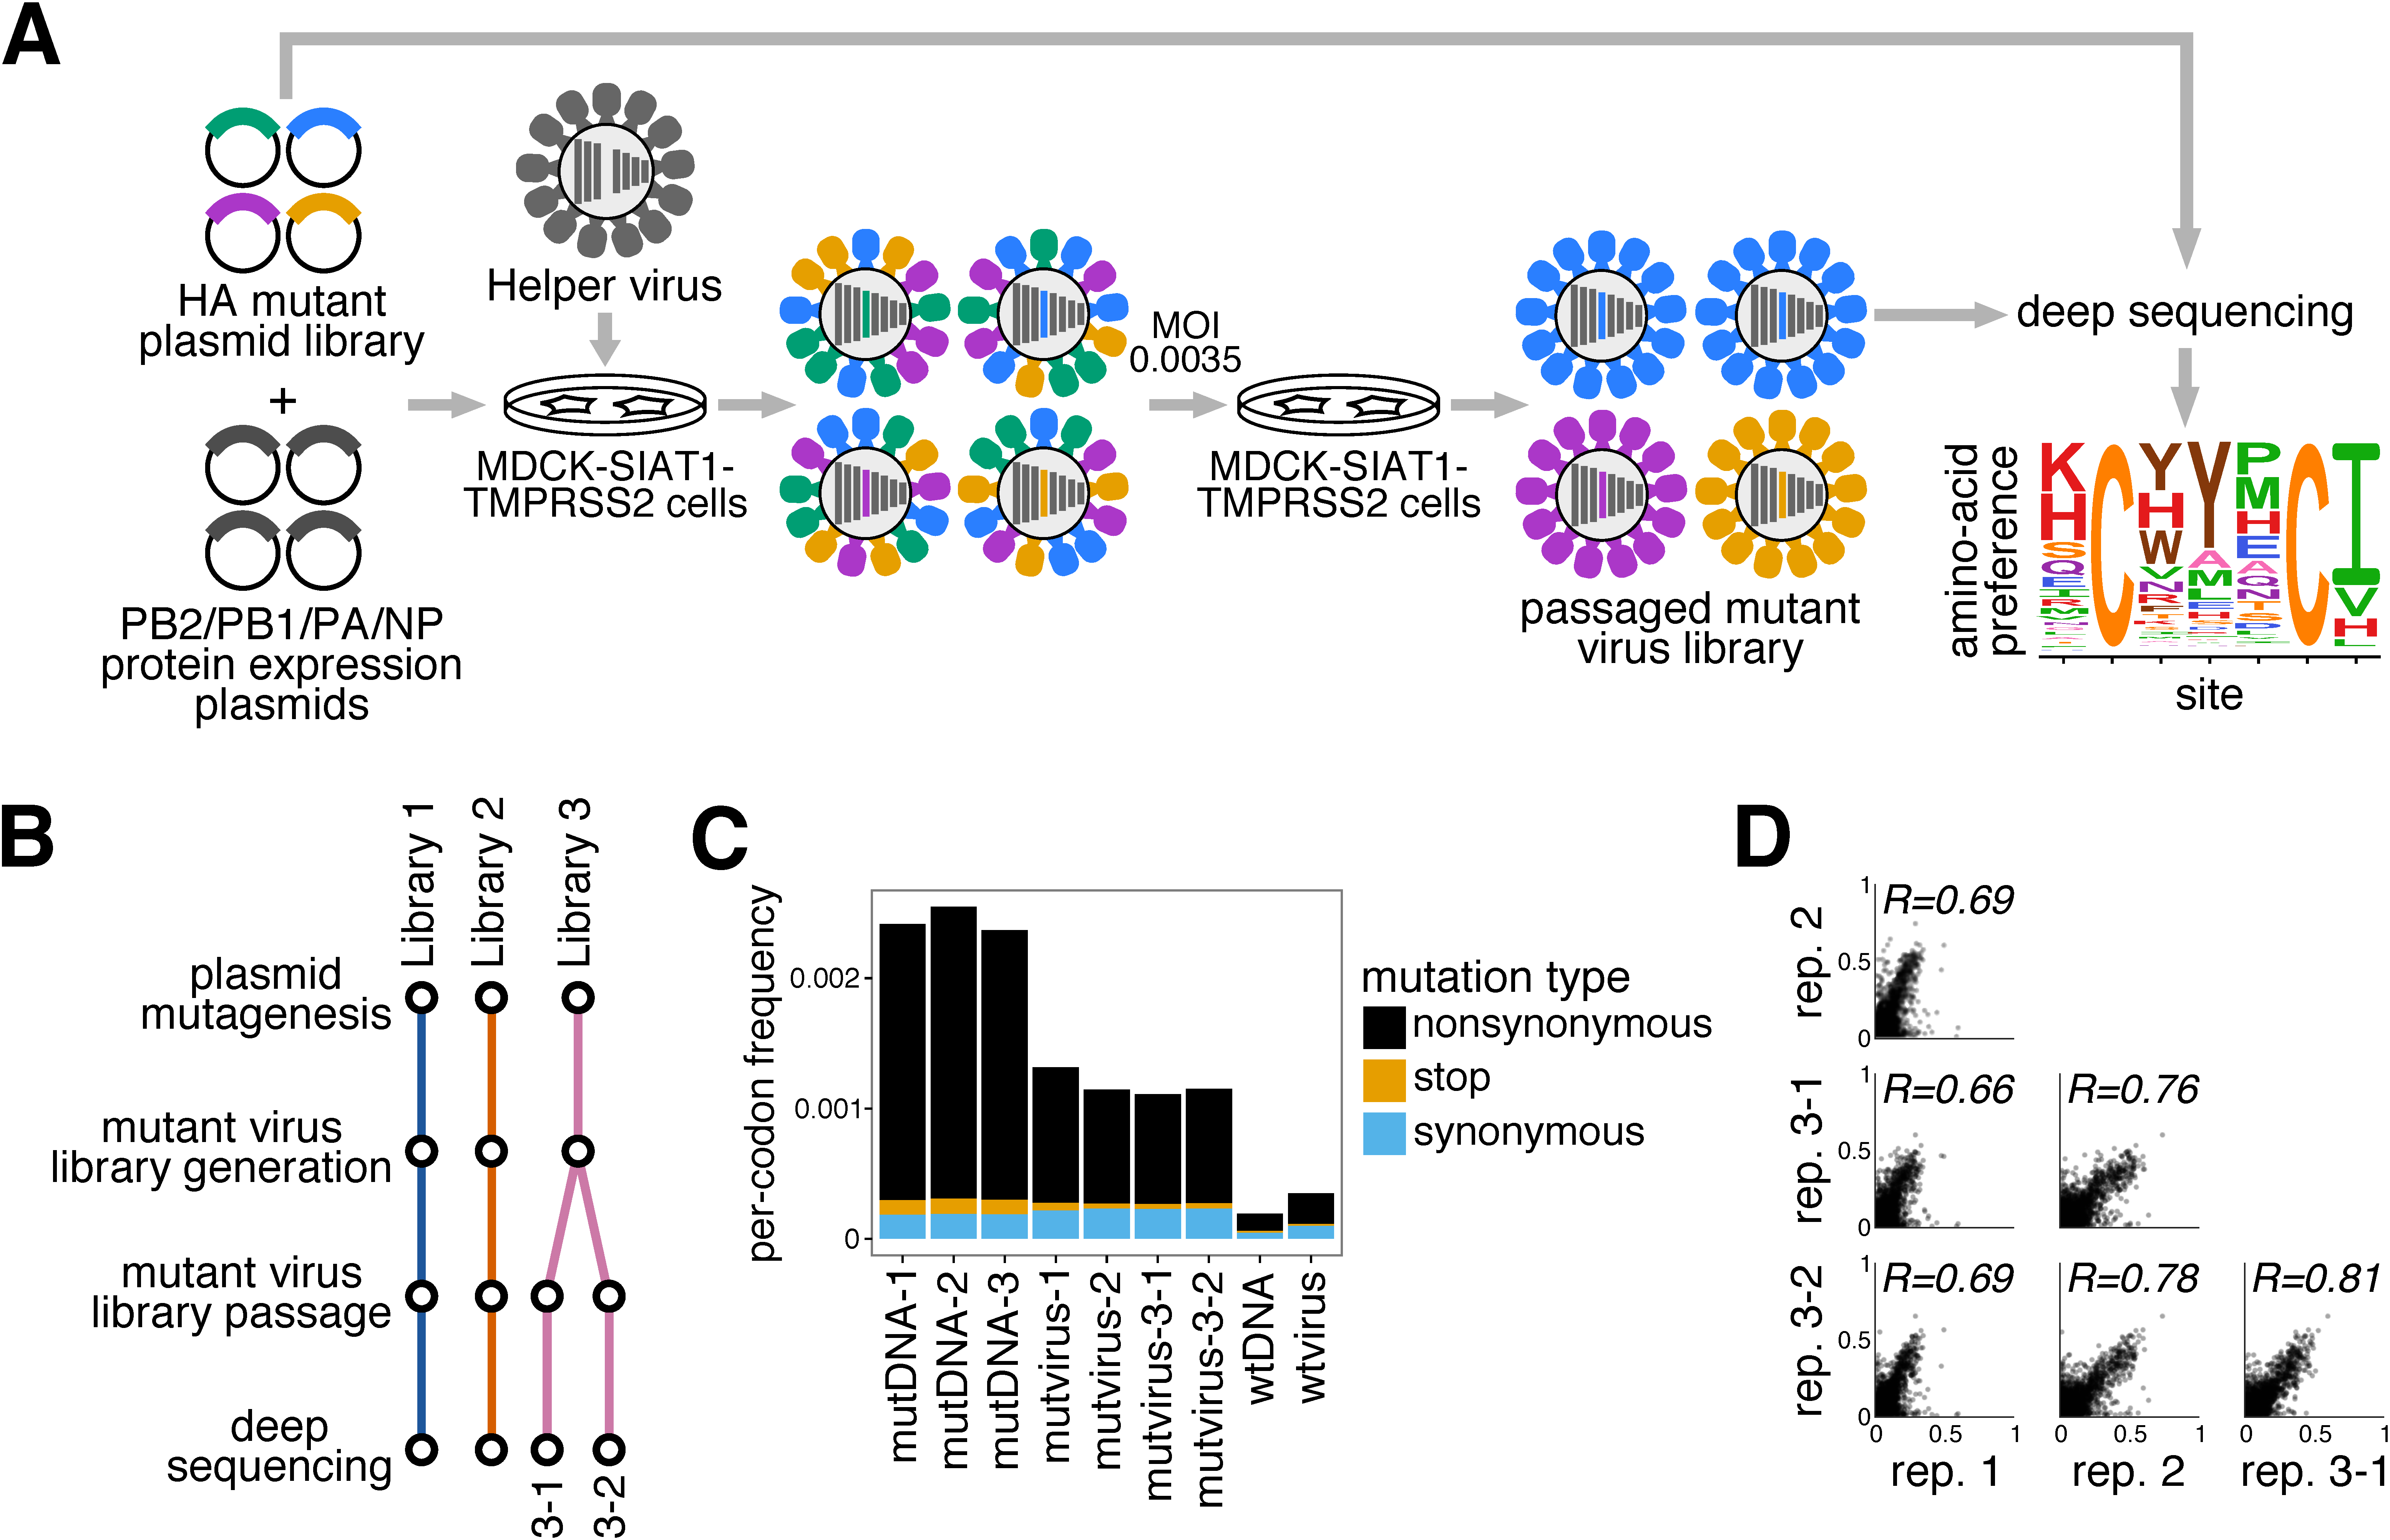
\includegraphics[width=12cm]{figs/dms_overview/dms_overview.pdf}
\caption{\label{fig:dms_overview}
{\bf Deep mutational scanning of the Perth/2009 H3 HA.}
(A) We generated mutant virus libraries using a helper-virus approach~\cite{doud2016accurate}, and passaged them at low MOI to establish a genotype-phenotype linkage and to select for functional HA variants. 
Deep sequencing of the variants before and after selection allowed us to estimate each site's amino-acid preferences.
(B) The experiments were performed in full biological triplicate. 
We also passaged and deep sequenced library 3 in duplicate.
(C) Frequencies of nonsynonymous, stop, and synonymous mutations in the mutant plasmid DNA, the passaged mutant viruses, and wildtype DNA and virus controls. 
(D) The Pearson correlations among the amino-acid preferences estimated in each replicate. 
}
\end{SCfigure*}

We next quantified the reproducibility of our deep mutational scanning measurements across biological and technical replicates. 
We first used the deep sequencing data for each replicate to independently estimate the preference of each site in HA for all 20 amino acids using the method described in~\cite{bloom2015software}.
Because there are 567 residues in HA, there are $567 \times 20 = 11,340$ estimated amino-acid preferences.
The correlations of the amino-acid preferences between pairs of replicates are shown in Figure~\ref{fig:dms_overview}D.
The biological replicates are fairly well-correlated, with Pearson's $R$ ranging from 0.69 to 0.78. 
Replicate 1 exhibited the lowest correlation with the other replicates, consistent with the observation that this replicate also showed the weakest selection against stop and nonsynonymous mutations perhaps indicating more experimental noise.
The two technical replicates 3-1 and 3-2 were only slightly more correlated than pairs of biological replicates, suggesting that bottlenecking of library diversity after the reverse-genetics step contributes most of the experimental noise.

\subsection*{Our measurements are consistent with existing knowledge about HA's evolution and function}
How do the HA amino-acid preferences measured in our experiments relate to the evolution of H3N2 influenza virus in nature?
This question can be addressed by evaluating how well an experimentally informed codon substitution model (ExpCM) using our measurements describe H3N2 evolution compared to standard phylogenetic substitution models~\cite{bloom2017identification,hilton2017phydms}.
Table~\ref{tab:phydms} shows that the ExpCM using the replicate-average measurements greatly outperforms conventional substitution models, showing that our experiments authentically capture some of the constraints on HA evolution. 
Note that while the relative ratio of nonsynonymous to synonymous substitutions (dN/dS or $\omega$) is $\ll$1 for conventional substitution models, this ratio is close to one for the ExpCM that accounts for the constraints measured in the experiments.
ExpCM contain a stringency parameter that relates the selection in the experiments to that in nature~\cite{bloom2017identification,hilton2017phydms}.
We fit a stringency parameter of 2.44 (Table~\ref{tab:phydms}), indicating that natural selection favors the same amino acids as the experiments, but with greater stringency.
Throughout the rest of this paper, we use experimental measurements re-scaled~\cite{bloom2017identification,hilton2017phydms} by this stringency parameter.
These re-scaled preferences are shown in Figure~\ref{fig:logoplot}.

\begin{table*}
\caption{\label{tab:phydms}
{\bf Substitution models informed by the experiments describe H3N2's natural evolution better than traditional substitution models.}}
\begin{center} 
\begin{tabular}{cccccccc}
\hline
\bf{Model} & \bf{$\Delta$AIC} & \bf{Log Likelihood} & \bf{Stringency} & \bf{$\omega$}  \\ \hline
ExpCM & 0.0 & -8439.33 & 2.44 & 0.91 \\
Goldman-Yang M5 & 2166.06 & -9516.36 & -- & 0.30, 0.84, 0.36 \\
ExpCM, averaged across sites & 2504.18 & -9691.42 & 0.68 & 0.32 \\
Goldman-Yang M0 & 2607.92 & -9738.29 & -- & 0.31 \\
\hline
\end{tabular}
 \end{center}
\addtabletext{Maximum likelihood phylogenetic fit to an alignment of human H3N2 influenza HAs using ExpCM~\cite{hilton2017phydms}, ExpCM in which the experimental measurements are averaged across sites, and the M0 and M5 versions of the Goldman-Yang model~\cite{yang2000codon}.
Models are compared by AIC~\cite{posada2004model}.
The $\omega$ parameter is dN/dS for the Goldman-Yang models, and the relative dN/dS after accounting for the measurements for the ExpCM.
For the M5 model, we give the shape parameter, rate parameter, and mean of the gamma distribution over $\omega$.
}
\end{table*}

A closer examination of Figure~\ref{fig:logoplot} reveals that the experimentally measured amino-acid preferences generally agree with existing knowledge about HA's structure and function.
For instance, sites that form structurally important disulfide bridges (sites 52 \& 277, 64 \& 76, 97 \& 139, 281 \& 305, 14 \& 137-HA2, 144-HA2 \& 148-HA2)~\cite{waterfield1981disulphide} possess high preference for cysteine.
At residues involved in receptor binding, there are strong preferences for the amino acids that are known to be involved in binding sialic acid, such Y98, D190, W153, and S228~\cite{weis1988structure,martin1998studies,nobusawa2000change}\comment{These old citations are for X-31 HA, you might also see if Paulson and/or Ian Wilson have newer structural papers on receptor-binding in recent H3 -- if so, add them}.
A positively charged amino acid at site 329 is important for cleavage activation of the HA0 precursor, and indeed this site exhibits a high preference for arginine~\cite{kido1992isolation, stech2005new}.
However, a notable exception occurs at the start codon at position -16, which does not show a strong preference for methionine. 
This codon is part of the signal peptide and is cleaved from the mature HA protein.
One possible reason we do not see a strong preference for methionine at this site is due to alternative translation-initiation at a downstream or upstream start site, as has been described for other HAs~\cite{girard2011upstream}.
% No upstream or downstream "ATG"'s are present. I did find an in-frame "ATC" one codon upstream of the canonical start site (in the non-coding region), and interestingly, all Perth/2009 HA sequences deposited in GenBank have an "ATT" in this non-coding position, including Seema's Perth HA.
% I6M(HA2) mutant slightly increases the fusion pH (Daniels 1985 Cell)
% We see high preference for T,S,Q over the wildtype Ile at site 226. Although Q226 in an H3 background is characterized as having preference for avian-type receptors, most of these studies were done in older H3 strains such as Aichi. Wu 2017 Cell Host Microbe has shown extensive epistasis in the RBS, specifically in the 220-loop, so perhaps the amino acids tolerated in this loop have shifted over time. Indeed the wildtype amino acids at 225 and 226 are different in Perth compared to HK68 and Aichi.

\begin{figure*}
\centering
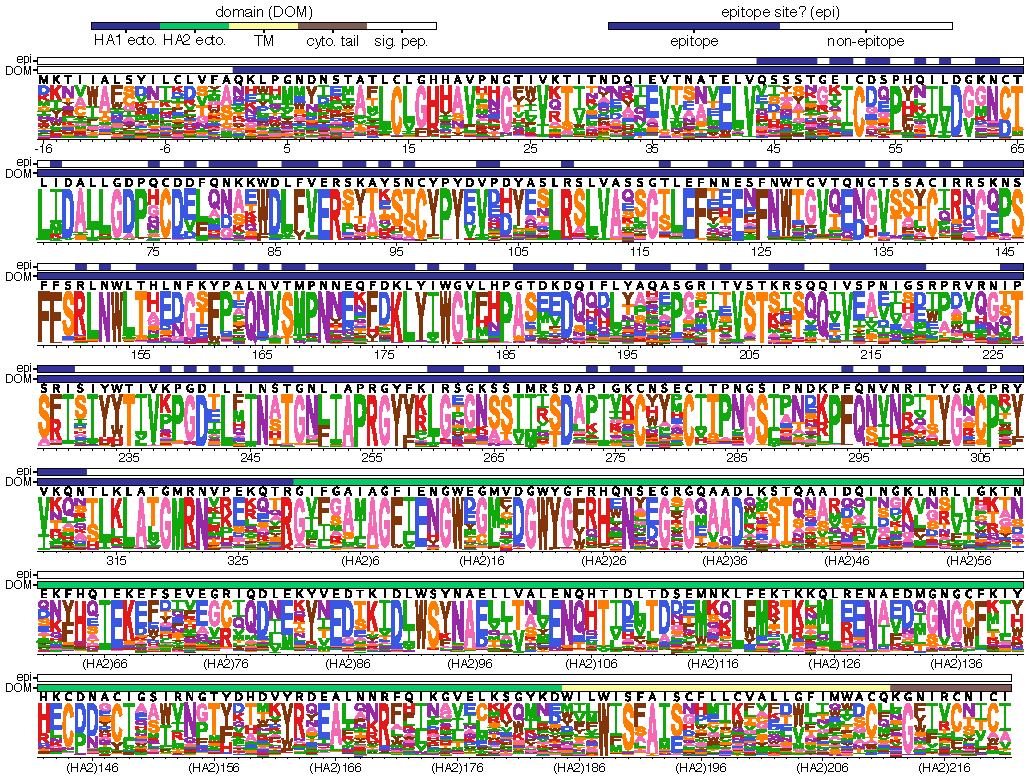
\includegraphics[width=17cm]{figs/prefslogoplot/rescaled-avgprefs_prefs.pdf}
\caption{\label{fig:logoplot}
{\bf The site-specific amino-acid preferences of the Perth/2009 HA measure in our experiments.}
The height of each letter is the preference for that amino acid, after taking the average of our experimental replicates and re-scaling~\cite{hilton2017phydms} by the stringency parameter in Table~\ref{tab:phydms}.
The sites are in H3 numbering.
The top overlay bar indicates whether or not a site is part of the set of epitope residues delineated in \cite{wolf2006long}
The bottom overlay bar indicates the HA domain (sig. pep. = signal peptide, HA1 ecto. = HA1 ectodomain, HA2 ecto. = HA2 ectodomain, TM = transmembrane domain, cyto. tail. = cytoplasmic tail).
The letters directly above each logo stack indicate the wildtype amino acid at that site.
}
\end{figure*}

\subsection*{There is less difference in mutational tolerance between the HA head and stalk domains for H3 than for H1}
Our experiments measure which amino acids are tolerated at each HA site under selection for protein function.
We can therefore use our experimentally measured amino-acid preferences to calculate the inherent mutational tolerance of each site, which we define as the Shannon entropy of the re-scaled preferences.
In prior mutational studies of the WSN/1933, the stalk domain of this H1 HA was found to be substantially less mutationally tolerant than its globular head~\cite{thyagarajan2014inherent,doud2016accurate}.

We performed a similar analysis using the current data for the Perth/2009 H3 HA.
Surprisingly, there was much less contrast in mutational tolerance between the stalk and head domains for the H3 HA than for the H1 (Figure~\ref{fig:mut_tolerance}).
For instance, the in H3 HA, the short helix A in the stalk is very mutationally tolerant.
Interestingly, more studies have reported selecting escape mutants from broadly neutralizing anti-stalk antibodies in H3~\cite{ekiert2011highly, friesen2014common, chai2016two, yamayoshi2017human} than in H1~\cite{okuno1993common,doud2017quantifying} HAs.

We also see high mutational tolerance in many of the known antigenic regions of H3 HA~\cite{wiley1981structural}.
For instance, in recent H3N2 strains, antigenic region B is immunodominant and the location of most major antigenic drift mutations~\cite{chambers2015identification,koel2013substitutions,popova2012immunodominance}.
We find that the most distal portion of the globular head near the 190-helix, which is part of antigenic region B, is highly tolerant of mutations (Figure~\ref{fig:mut_tolerance}).
Antigenic region C is also notably mutationally tolerant.

Many residues inside HA's receptor binding pocket are known to be highly functionally constrained~\cite{wilson1981structure,martin1998studies}, and our data indicates that these sites are relatively mutationally intolerant in both H3 and H1 HAs.
In contrast, the residues surrounding the receptor binding pocket are fairly mutationally tolerant, which may contribute to the rapidity of influenza's antigenic evolution, as these sites are under strong immune pressure.~\cite{wiley1981structural,koel2013substitutions}.

\begin{SCfigure*}[\sidecaptionrelwidth][t]
\centering
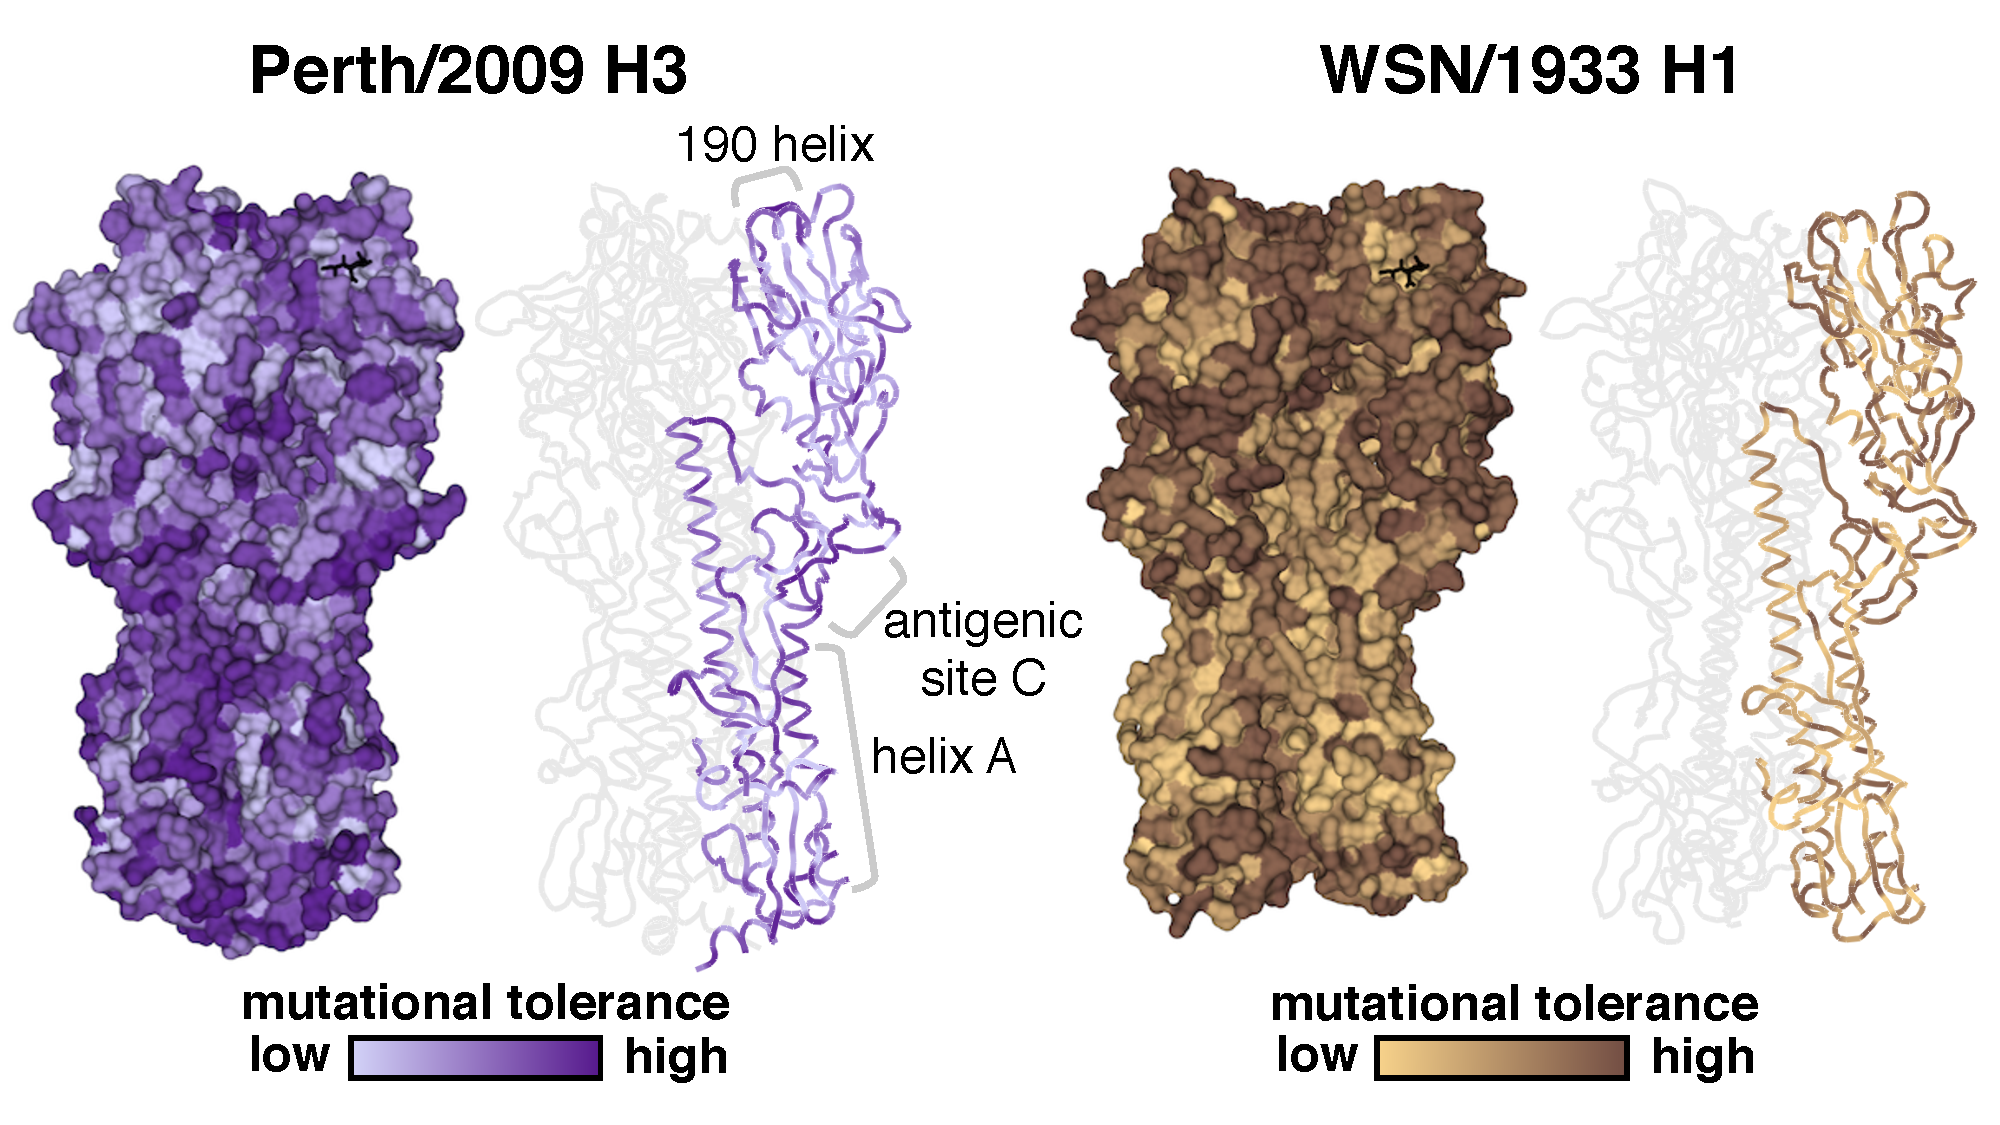
\includegraphics[width=11.4cm]{figs/mut_tolerance/entropy_heatmap.pdf}
\caption{\label{fig:mut_tolerance}
{\bf Mutational tolerance of each site in H3 and H1 HAs.}
Mutational tolerance as measured in the current study is mapped onto the structure of the H3 trimer (PDB 4O5N;~\cite{lee2014receptor}).
Mutational tolerance of the WSN/1933 H1 HA as measured in \cite{doud2016accurate} is mapped on the structure of the H1 trimer (PDB 1RVX;~\cite{gamblin2004structure}).
Different color scales are used because measurements are comparable among sites within the same HA, but not necessarily across HAs.
Both trimers are shown in approximately the same orientation. 
For each HA, the structure at left shows a surface representation of the full trimer, while the structure at right side shows a ribbon representation of just one monomer.
The sialic acid receptor is shown in black sticks.
}
\end{SCfigure*}

\subsection*{The experimental measurements can help discriminate between successful and unsuccessful influenza virus lineages}
A major goal in the study of rapidly evolving viruses such as influenza is to forecast evolutionary trajectories\comment{Michael Lassig has a Nature Ecology \& Evolution review}.
For instance, forecasting which viral lineages will dominate the upcoming influenza season is an integral part of vaccine-strain selection\comment{add reference}. 
Evolutionary forecasts must ultimately distinguish between successful and unsuccessful viral lineages, which in the case of human influenza virus means distinguishing between the trunk and side branches of the phylogenetic tree (Figure~\ref{fig:H3N2_phylogeny}).

To investigate whether our experiments can aid in distinguishing trunk and side branch lineages, we calculated the experimentally measured effects of all mutations in a maximum-likelihood reconstruction of the phylogeny in Figure~\ref{fig:H3N2_phylogeny}.
The mutations that occurred on the trunk of the tree were consistently more beneficial for viral growth according to our experimental measurements (Figure~\ref{fig:trunkvssidebranch}A).
This difference in the effects of mutations between the trunk and side branch lineages was statistically significant when taken across the entire phylogeny (Figure~\ref{fig:trunkvssidebranch}B).
Some influenza sequences are determined using egg- or cell-passaged isolates that contain lab-adaptation mutations~\citep{wu2017structural,mcwhite2016sequence,skowronski2016mutations}.
These mutations will largely occur on the terminal side branches that lead to tip nodes on the phylogenetic tree.
We therefore re-calculated the statistics separating side branches to tip and internal nodes, and again found that the difference between the trunk and both sets of side branches was statistically significant (Figure~\ref{fig:trunkvssidebranch}B).
Therefore, strains with mutations that we experimentally measure to be favorable for viral replication tend to do better in nature than strains with mutations that we measure to be less favorable. 

Our experiments were performed on the Perth/2009 HA, but we are scoring mutations on a phylogenetic tree that extends from 1968 to 2017.
Because the effects of mutations can vary with genetic background\comment{cite some papers about epistasis, amino-acid shifts, etc}, it is possible that the effects of mutations that we measured in the Perth/2009 HA might have shifted somewhat in other related HAs.
To explore this question, we scored the complete HA sequence of every node in the phylogenetic tree by quantifying its average per-site sequence preference for HA sequence $\mathbf{s}$, which is defined as 
\begin{equation}
F\left(\mathbf{s}\right) = \frac{1}{L}\displaystyle\sum_{r=1}^L \ln \pi_{r, s_r},
\end{equation}
where $\pi_{r, a}$ is the preference for amino-acid $a$ at site $r$ as measured in our experiments (e.g., Figure~\ref{fig:logoplot}), $s_r$ is the amino-acid at site $r$ in HA sequence $\mathbf{s}$, and $L$ is the length of the sequence.
Figure~\ref{fig:trunkvssidebranch}C shows that the sequences of trunk nodes tend to be more highly preferred than those of side branch nodes across the entire timespan, consistent with the finding that trunk mutations are generally more favorable than side branch mutations. 
However, the average per-site sequence preference increases as the nodes approach the Perth/2009 strain.
The Perth/2009 itself has among the highest per-site sequence preference of the entire tree, despite falling on a side branch.
These results suggest that there is some HA background-dependence in the effects of mutations, but that despite this fact our experimental measurements consistently reveal the selective advantage of the trunk over a more than half-century of viral evolution.


\begin{figure}
\centering
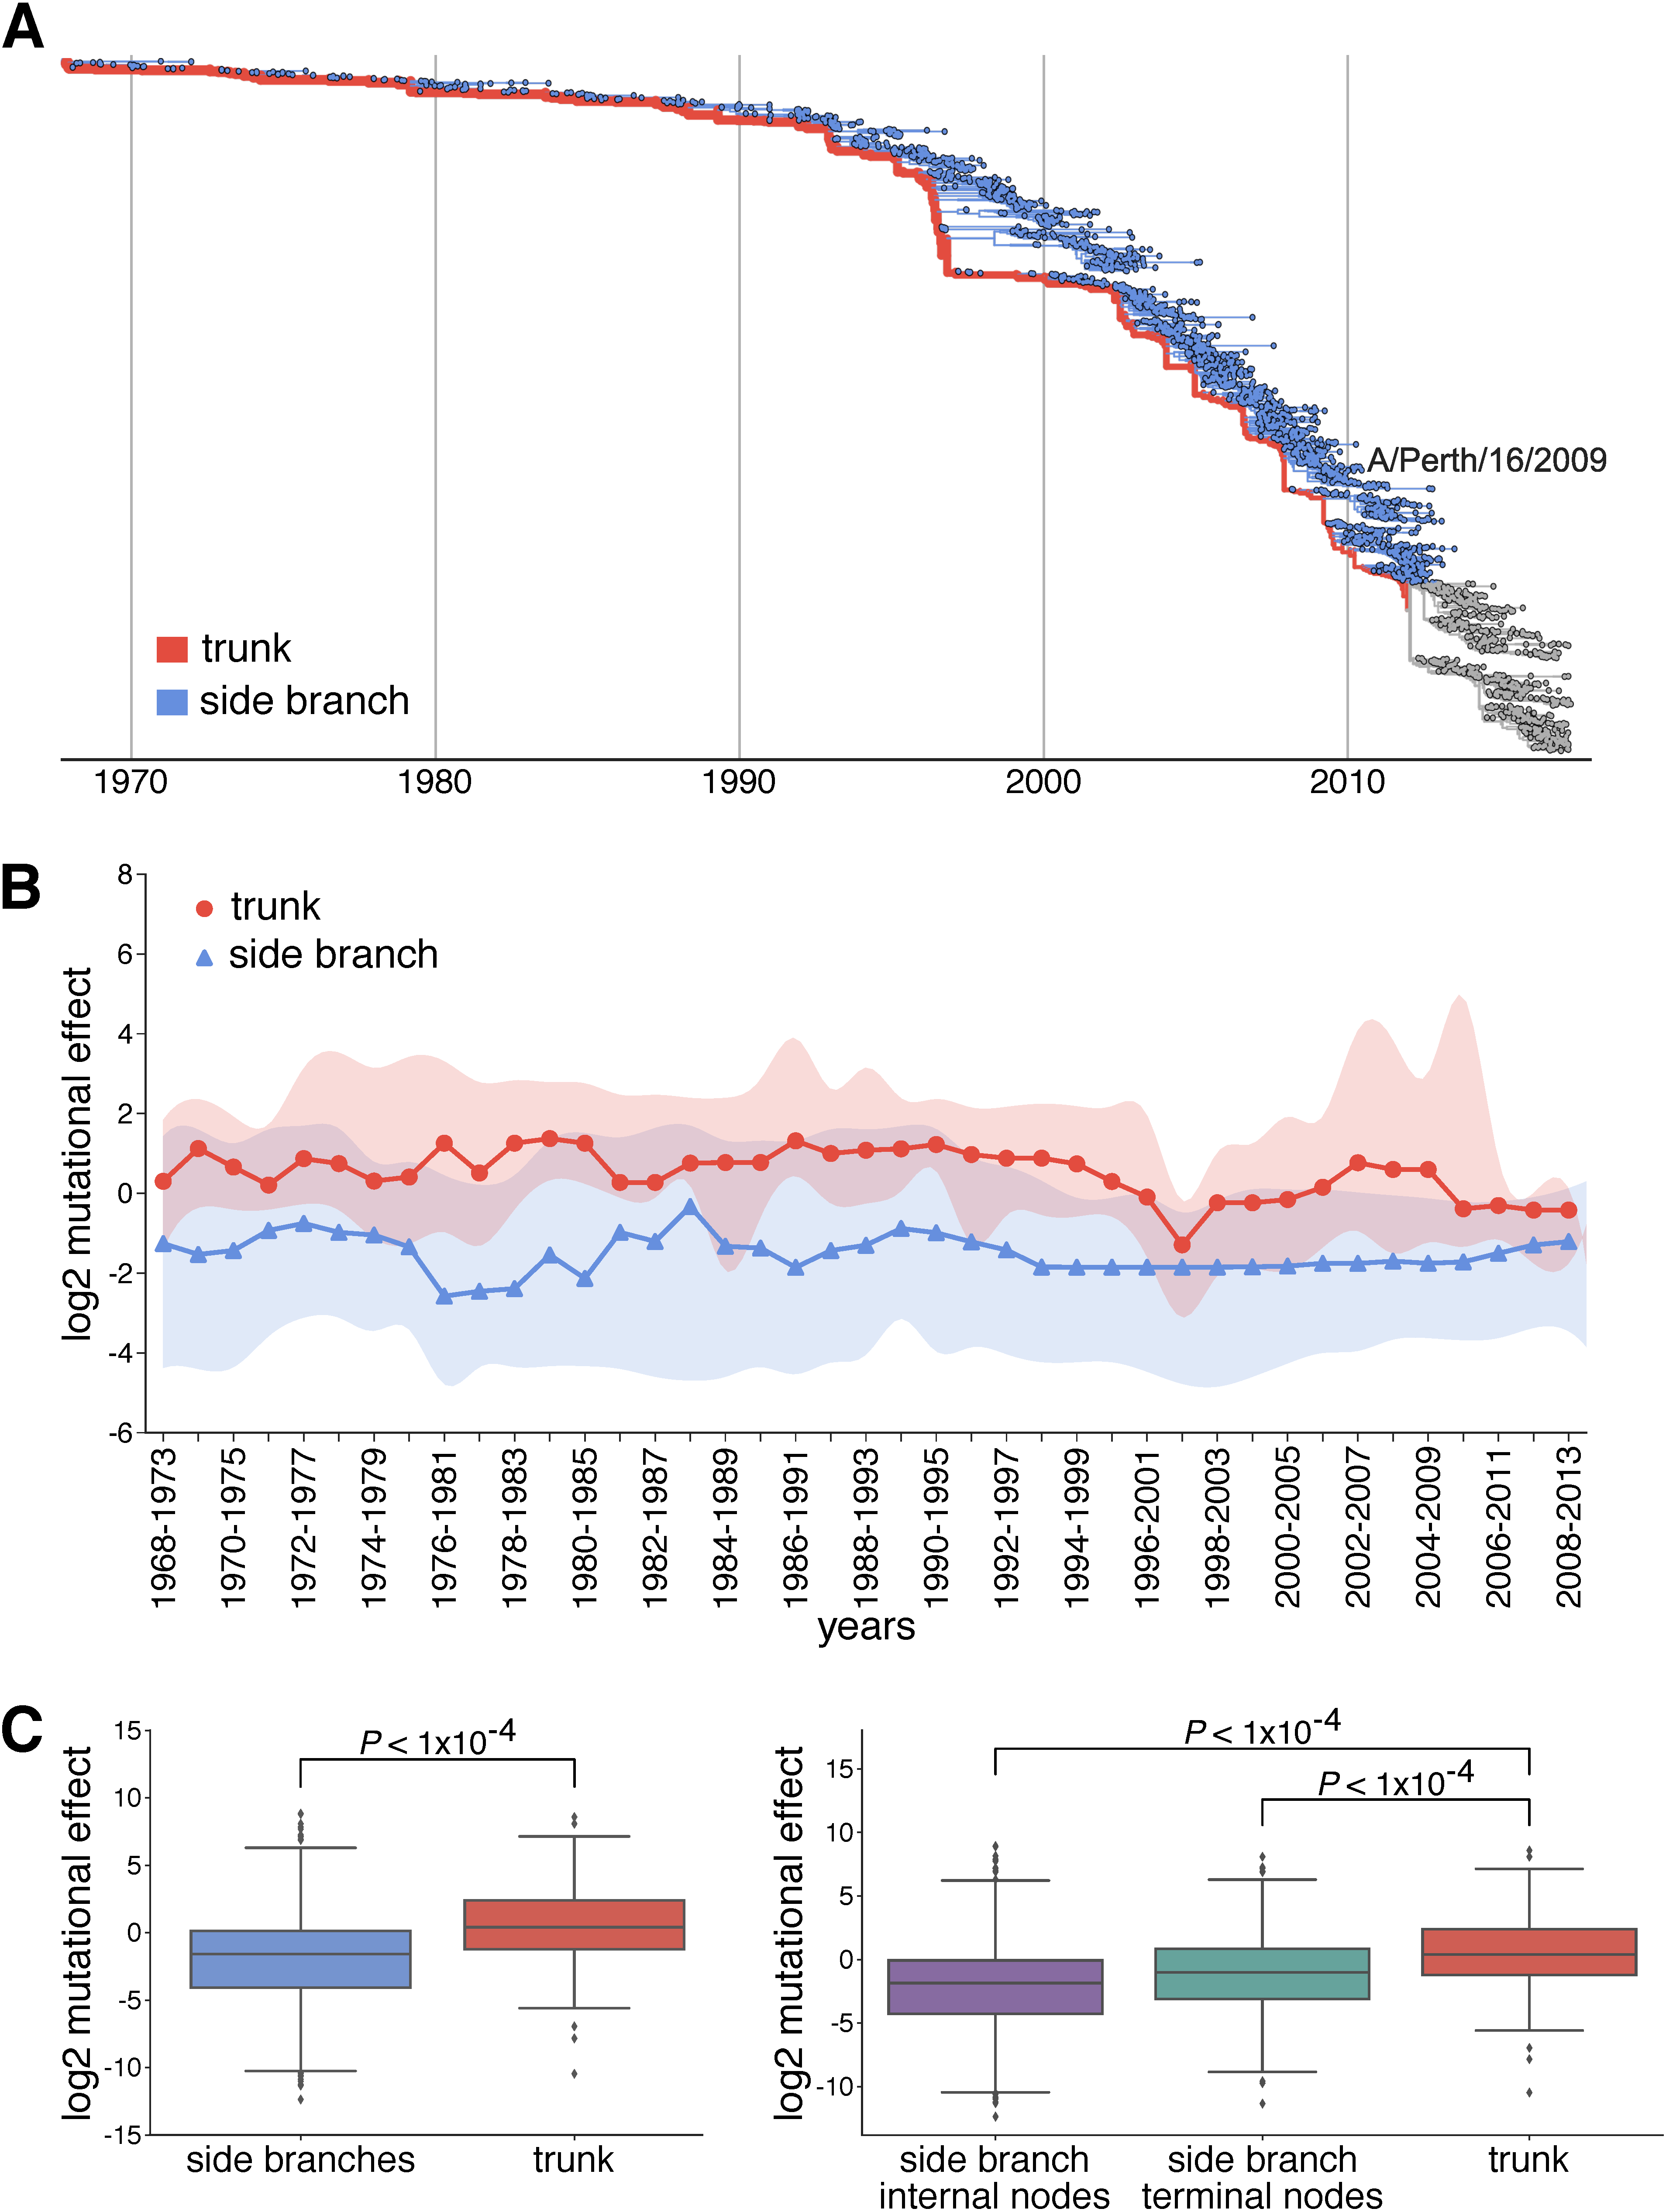
\includegraphics[width=\columnwidth]{figs/trunkvssidebranch/trunkvssidebranch.pdf}
\caption{\label{fig:trunkvssidebranch}
{\bf Mutations on the trunk are more favorable than those on the side branches according to our experimental measurements.}
\comment{Legend will be written under assumption that panels (B) and (C) are swapped. Also add sequence preference \emph{per site} to y-axis of the new (C).}
(A) We used our experiments to calculate the log$_{2}$ mutational effect for all trunk and side branch mutations in five-year windows from 1968 to 2013. 
The central year in each window is denoted on the x-axis.
Median mutational effects in each window are shown as circles for the trunk and triangles for side branches. 
The shaded regions demarcate the interquartile range.
Negative numbers signify mutations towards less preferred amino acids, while positive numbers signify mutations to more preferred mutations.
(B) The log$_{2}$ mutational effect for all side branch and all trunk mutations (left panel), and the same data but separating side branches to terminal and internal nodes.
$P$-values were computed by randomizing the experimental measurements among sites 10,000 times, and determining how often the difference in median mutational effect between the trunk and side branches for the randomized data exceeded the actual value.
(C) The average per-site sequence preference of every node in the phylogenetic tree in Fig.~\ref{fig:H3N2_phylogeny}.
Trunk nodes are in red, side branch nodes in blue, and Perth/2009 is marked with a yellow star.
More preferred sequences have larger values.
}
\end{figure}

\subsection*{Our experiments suggest different patterns of evolution at epitope and non-epitope sites}
HA is under selection both to maintain its essential function in viral growth and to escape pre-existing immunity.
Most of the immune selection is focused on a subset of so-called ``epitope sites'' that are targets of the immunodominant antibody response.
Although both epitope and non-epitope sites evolve rapidly, immune selection drives a higher rate of evolution at epitope sites.
In the timeframe from 1968 to 2012, the trunk of the tree in Figure~\ref{fig:H3N2_phylogeny} fixed \comment{X} epitope mutations per site, but only Y non-epitope mutations per site.
Since our experiments only measure how mutations affect viral growth, they might be expected to describe the evolution of epitope and non-epitope sites differently.

Mutations that occur on the trunk are scored as significantly more favorable in our experiments than side-branch mutations at both epitope and non-epitope sites (Figure~\ref{fig:sequence_preference}A).
Therefore, our experiments can distinguish evolutionarily favorable mutations both at sites that are predominantly under functional constraint and ones that are also under immune pressure.
The fact that our experiments can discriminate between the trunk and side branch at epitope sites despite only assaying for viral growth underscores the fact that most epitope sites are still important for HA function\comment{cite?}. 

But interestingly, there are clear differences in how the average per-site sequence preference changes over time at the epitope and non-epitope sites (Figure~\ref{fig:sequence_preference}B).
The per-site sequence preference at epitope sites increases over time (Figure~\ref{fig:sequence_preference}A \comment{and new associated supplement that zooms in}), whereas at non-epitope sites it remains relatively constant.
In addition, the per-site sequence preference is consistently higher at non-epitope than epitope sites, perhaps consistent with the fact that strong immune selection can lead to the fixation of less functionally favorable mutations at epitope sites.
The fact that the epitope sites exhibit more of an increase in sequence preference over time may be due to the fact that they fix more mutations.
It is known that as mutations accumulate at protein sites, they can lead to epistatic shifts in the effects of mutations\comment{general epistasis appears}.
Such epistasis has been experimentally demonstrated for HA\comment{Yewdell paper, maybe Scott Hensley has something else}, including at some specific epitope sites in H3 HA~\cite{wu2017diversity}.
We hypothesize that the rapid evolution of epitope sites in HA leads to epistatic interactions that shift the effects of mutations, leading to an apparent increase in per-site sequence preference over time when mutational effects are measured in the Perth/2009 HA.

\begin{figure}
\centering
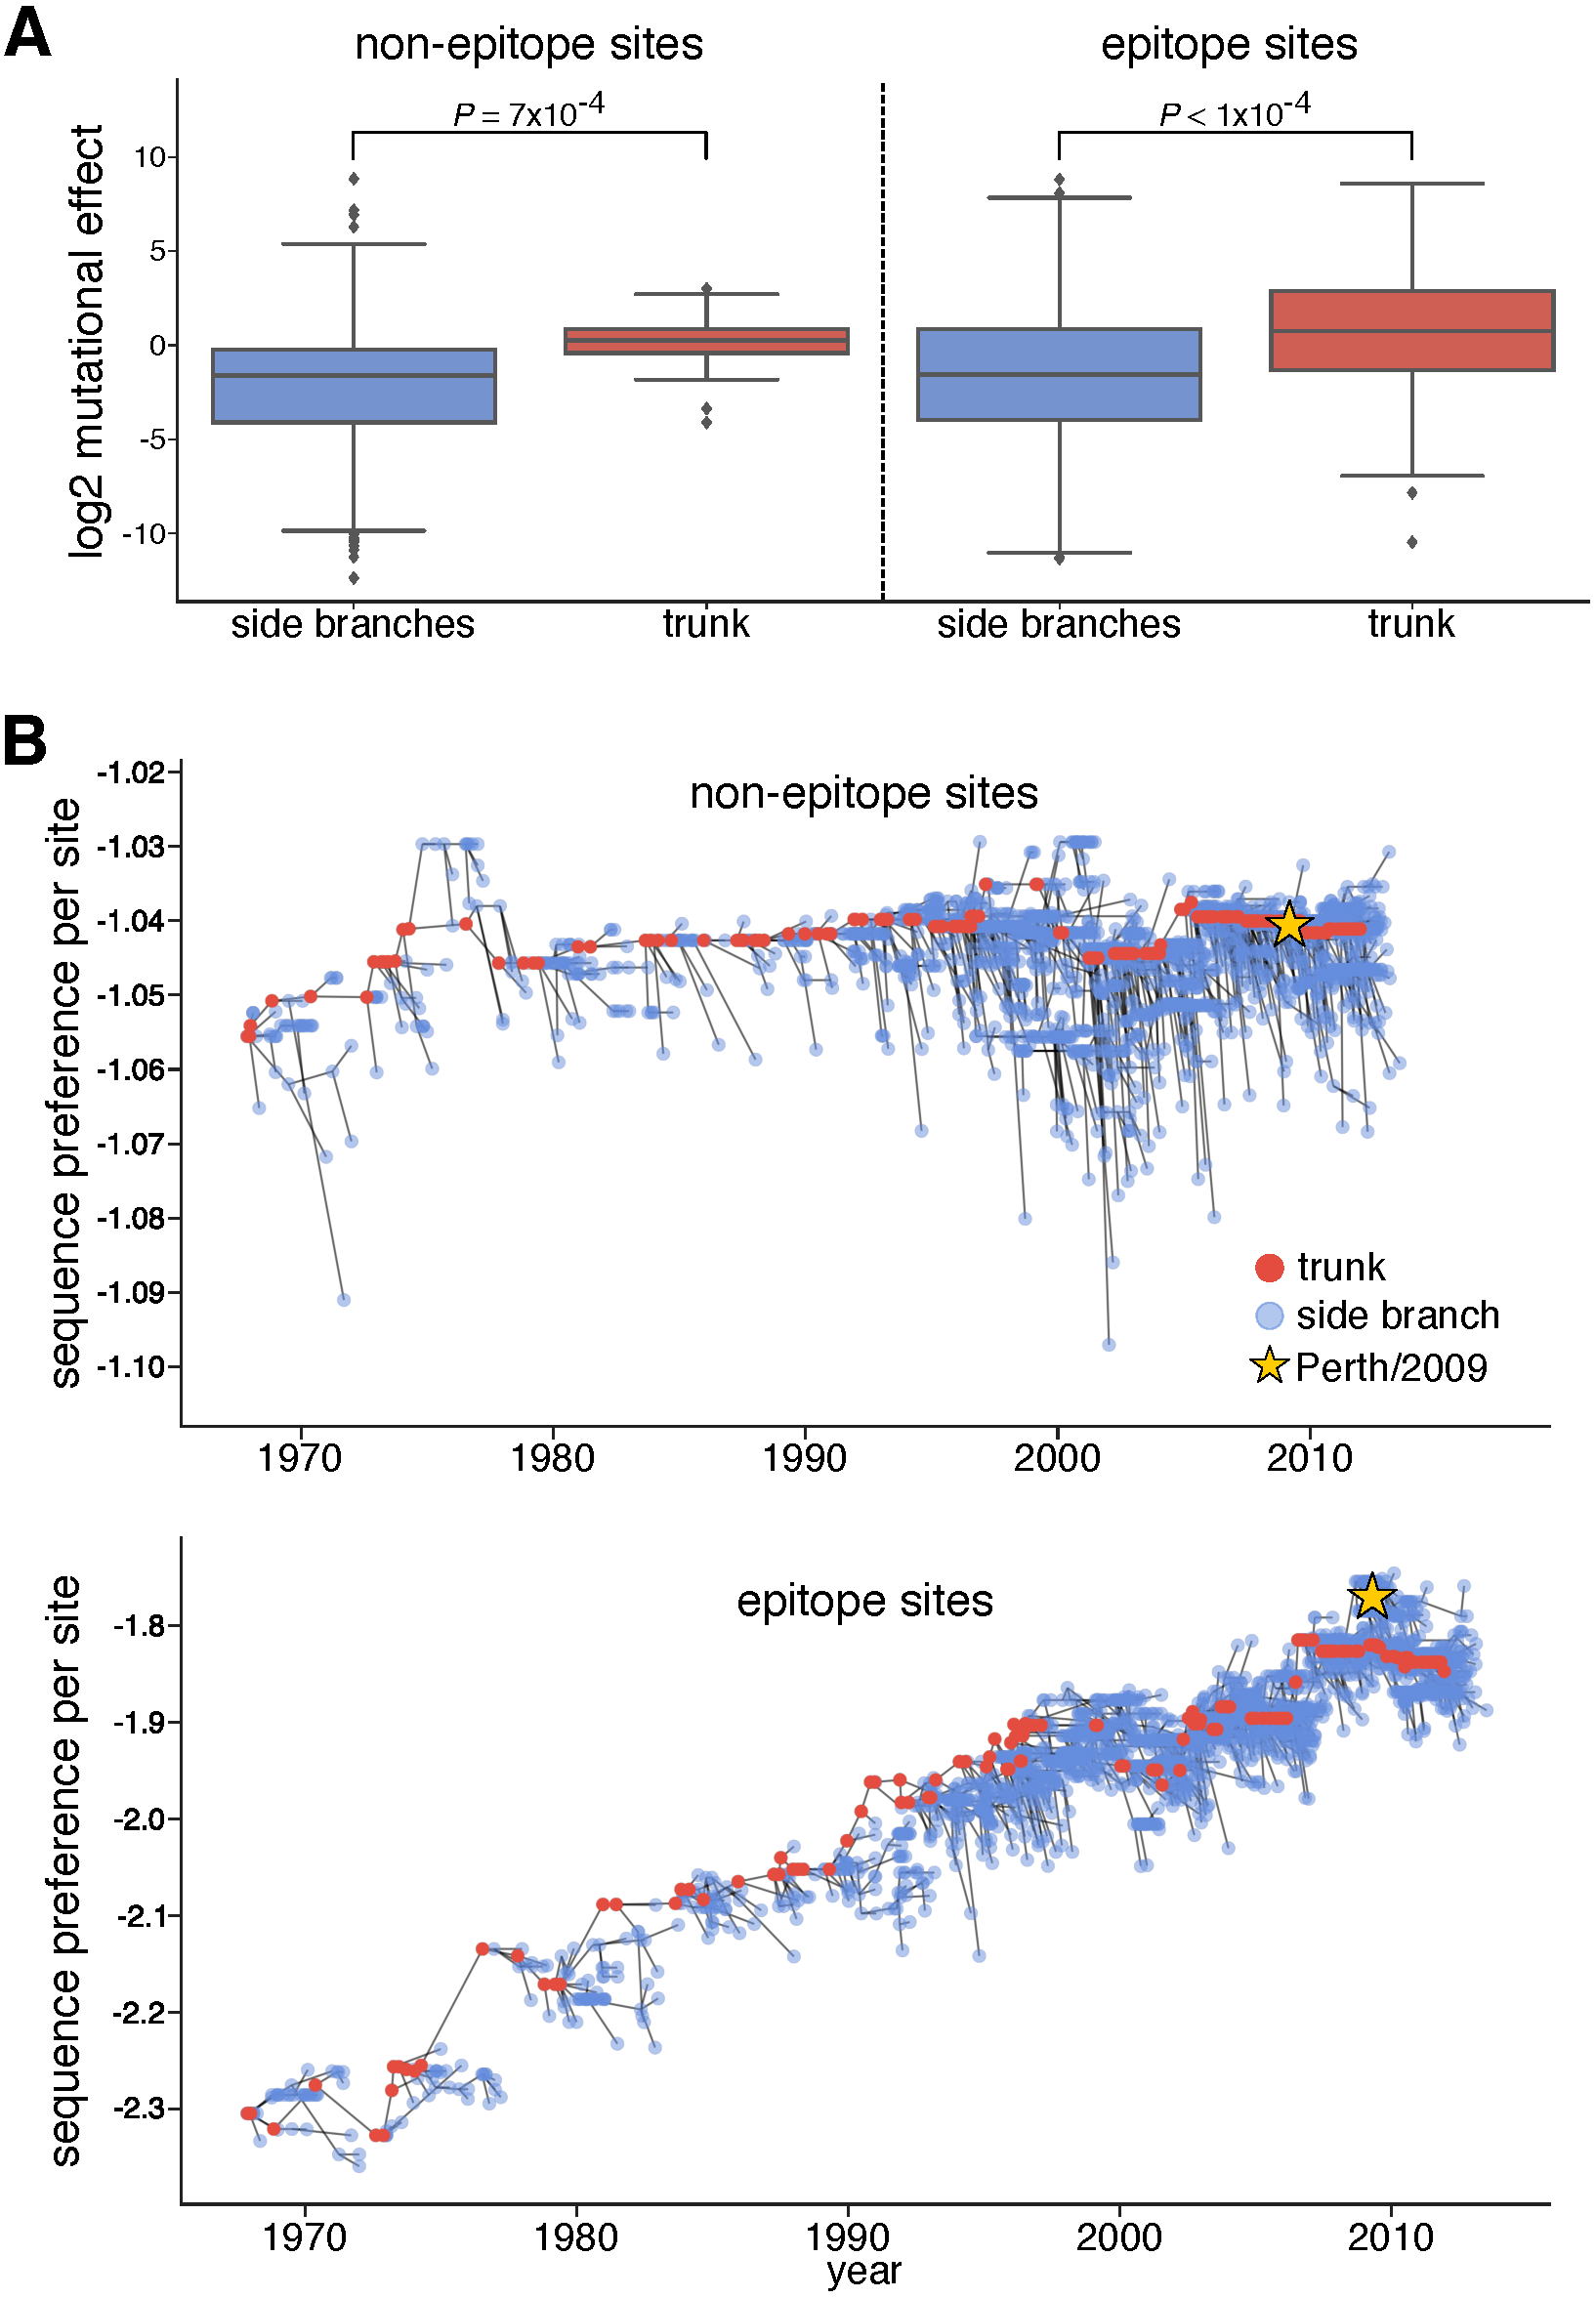
\includegraphics[width=\columnwidth]{figs/sequence_preference/sequence_preference.pdf}
\caption{\label{fig:sequence_preference}
\comment{Switch panels A and B, the legend is already written to reflect that.}
{\bf Effects of mutations at epitope and non-epitope sites during HA evolution.}
We partitioned HA into epitope and non-epitope sites using the definitions of Wolf \textit{et al}~\cite{wolf2006long}.
(A) The log$_{2}$ mutational effects for side branch and trunk mutations at non-epitope (left) and epitope (right) sites.
$P$-values were computed as in Figure~\ref{fig:trunkvssidebranch} but only performing the randomizations over the appropriate set of sites (non-epitope or epitope).
(B) 
The average per-site sequence preference for all nodes in the phylogenetic tree, calculated separately for each set of sites.
\comment{Write the P-value as $<10^{-4}$ if \emph{all} $10^4$ randomizations are less than the actual value. Otherwise write something like 0.0007 or (maybe if a lot of zeros $7\times10^{-4}$.
Add supplementary figure for the zoom-in of non-epitope sites and then refer to it in the Figure legend here. You could even just add the old figure that split them and shows both epitope and non-epitope on their own y-axis as the supplement.
I think the randomizations should be done just within the same set of sites.}
}
\end{figure}


\subsection*{Somehow merged into next subsection}

Can we then distinguish lineage-specific mutational effects using the preferences measured in a distantly related HA homolog?
We used the WSN/1933 H1 preferences measured in~\cite{doud2016accurate} to quantify the effects of H3 trunk and side branch mutations, shown in Figure~\ref{fig:WSN_trunkvssidebranch}.
It is evident that we do not see trunk mutations significantly more favored than side branch mutations, suggesting that our ability to discriminate successful and unsuccessful strains degrades over sufficiently long evolutionary distances. 

\begin{figure*}
\centering
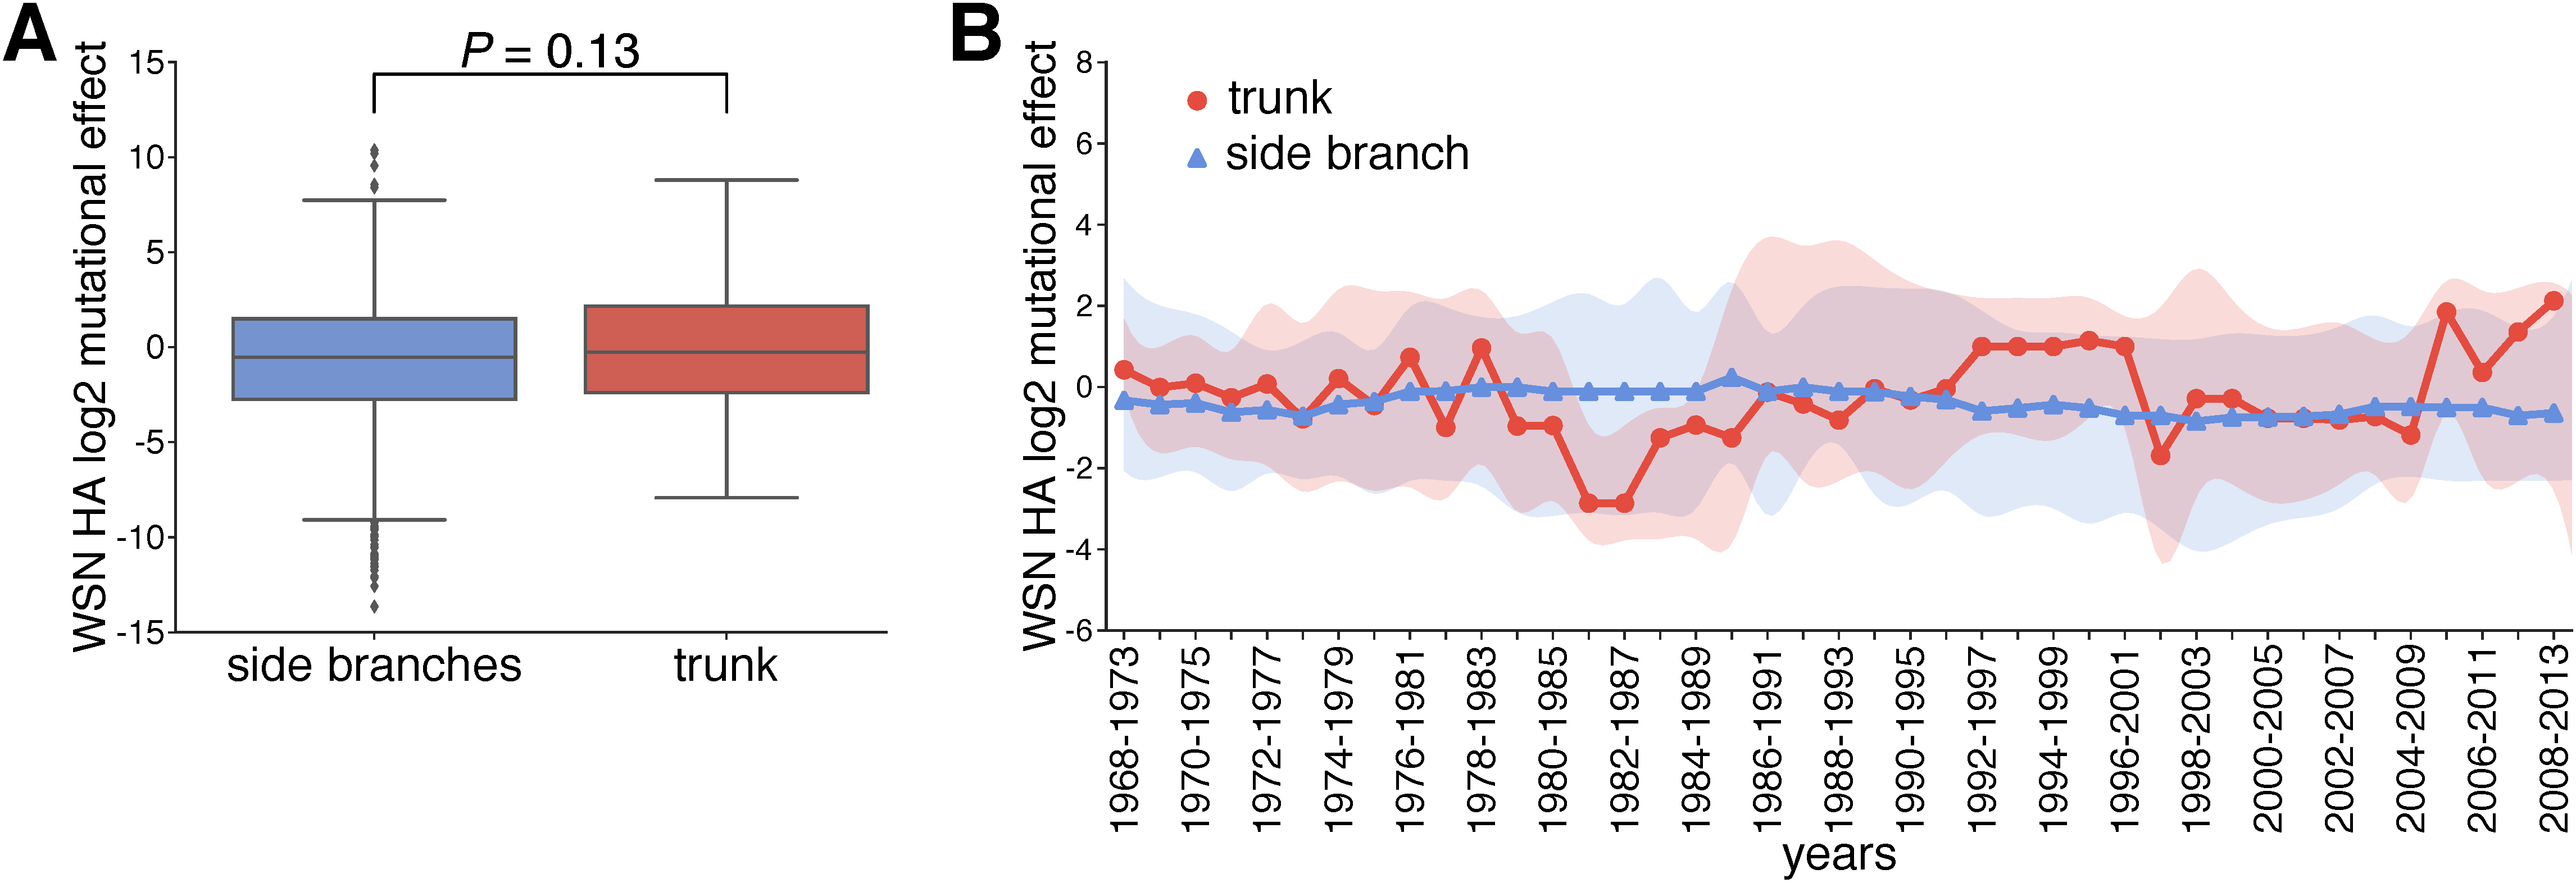
\includegraphics[width=15cm]{figs/WSN_trunkvssidebranch/WSN_trunkvssidebranch.pdf}
\caption{\label{fig:WSN_trunkvssidebranch}
{\bf The WSN/1933 H1 preferences do not reveal differences in trunk vs side branch mutational effects}
(A) We used the WSN/1933 H1 preferences experimentally measured in~\cite{doud2016accurate} to calculate the log$_{2}$ mutational effects of trunk and side branch mutations from the inferred H3N2 phylogeny in Figure~\ref{fig:trunkvssidebranch}.
(B) We also performed a sliding window analysis with the WSN/1933 H1 preferences.
}
\end{figure*}

\subsection*{The H1 and H3 preferences have shifted at many sites}
How shifted are the preferences between evolutionarily distant homologs such as H1 and H3?
Although we have previously compared the experimentally measured preferences between related protein homologs of NP~\cite{doud2015site} and of Env~\cite{haddox2017mapping}, the HA homologs we have studied are considerably more diverged than either of these pairs.
The WSN/1933 H1 and the Perth/2009 H3 fall into two phylogenetically distinct groups and share 42\% amino-acid identity (Figure~\ref{fig:distance_distribution}A), allowing us to examine what has shifted and what has remained conserved across such diverged homologs.
Simply correlating the preferences between H1 and H3 reveals that the replicate measurements within a homolog are more correlated than between homologs (Figure~\ref{fig:distance_distribution}B).

However, to quantify the extent of mutational shifts at a site-by-site level, we used an approach described in~\cite{doud2015site,haddox2017mapping}.
We aligned Perth/2009 H3 and WSN/1933 H1 and at each alignable site calculated the difference in preferences between homologs while correcting for experimental noise within homologs.
The distribution of shifts is shown in Figure~\ref{fig:distance_distribution}C.
Although many sites have small shifts near zero, a considerable number of sites have large shifts in preference, reaching a difference of 0.86 out of a maximum possible of 1.0.
When we compare HA to the preferences measured in the non-homologous protein HIV Env~\cite{haddox2017mapping}, nearly all sites are shifted.
On the other hand, when we randomize the HA replicates to generate a null distribution, there is very little shift in preferences. 
For comparison, the preferences of the HIV Env homologs, which are 86\% identical at the amino-acid level, are mostly similar. 
Although there are a small number of sites with larger shifts reaching a maximum of 0.52, we do not see a dramatic tail in the distribution as we see for the HA's.
These observations suggest that as protein homologs diverge, their preferences increasingly shift.

\begin{figure*}
\centering
\includegraphics[width=17cm]{figs/distance_distribution/distance_distribution.pdf}
\caption{\label{fig:distance_distribution}
{\bf The HA homologs exhibit many large shifts in preference compared to shifts for other viral protein homologs}
(A) A phylogenetic tree of the HA subtypes, with the two HA's, WSN/1933 H1 and Perth/2009 H3, for which we have measured amino-acid preferences denoted on the tree. 
The WSN/1933 H1 and the Perth/2009 H3 share $\sim$42\% amino-acid identity.
(B) The correlations of the amino-acid preferences for replicates both within and between the two HA homologs. 
The within-Perth/2009 and the within-WSN/1933 correlations are shown in purple and brown, respectively.
The between homolog correlations are in gray.
(C) The distribution of shifts in preference for various homolog pairs are shown.
The top two distributions show the distances between each of the HA homologs with the non-homologous HIV Env~\cite{haddox2017mapping}. %BF520
The center distribution shows the corrected distance between the two HIV Env homologs, which share 86\% amino-acid identity.
The fourth distribution from the top is a null generated by randomizing the HA replicates and computing the distances.
The bottom distribution is the corrected distance between the Perth/2009 H3 and WSN/1933 H1 homologs at all sites that align.
}
\end{figure*}

We next asked if shifted sites tend to cluster together in the HA structure.
However, the sites of large shifts were interspersed across HA and did not seem to obviously localize together (Figure~\ref{fig:RMSD_heatmap}A).
Yet, at the domain level, we found the stalk domain to be significantly less shifted than the globular head domain (Figure~\ref{fig:RMSD_heatmap}B). 
This is unsurprising given that the stalk domain is more conserved both within and across HA subtypes~\cite{nobusawa1991comparison,hai2012influenza,mallajosyula2014influenza}.
Sites absolutely conserved across all 18 HA subtypes were also found to be significantly less shifted than sites not conserved (Figure~\ref{fig:RMSD_heatmap}B), which is suggestive of the high functional importance of the sites that have remained unchanged throughout the divergence of HA.

Despite their large sequence divergence, H1 and H3 adopt nearly identical protein folds~\cite{ha2002h5,russell2004h1}.
Previous work has found that although the subdomain structures are highly similar, there are differences in the rotation and upward translation of the globular head subdomains relative to the central stalk domain among the four HA clades represented by H1 \& H5, H9, H7, and H3~\cite{ha2002h5,russell2004h1}.
One explanation for such clade-specific subdomain position differences could be local and/or long-range conformational interactions between sites that are variable between clades \comment{needs better wording}.
We would expect such sites to exhibit large shifts in preference.
Indeed, clade-specific sites that are conserved within the H1 clade (including H1, H2, H5, and H6) or within the H3 clade (including H3, H4, and H14) are significantly shifted compared to non-clade-specific sites.

In particular, the clade-specific upward shift of the globular head relative to the stalk has largely been attributed to the interaction between sites 107 and 75(HA2)~\cite{ha2002h5,russell2004h1}.
The H1 HA has a taller turn in the interhelical loop connecting helix A and helix B in the stalk domain, and this tall turn is stabilized by a hydrogen bond between Glu-107 and Lys-75(HA2) (Figure~\ref{fig:RMSD_heatmap}C).
In the WSN/1933 HA, site 107 has a high preference for Glu and 75(HA2) strongly prefers positively charged Lys and Arg.
In contrast, the interhelical loop in H3 HA makes a sharper and shorter turn which is facilitated by a Gly at 75(HA2).
This site prefers Gly and to a lesser extent Val, while site 107 is fairly tolerant of mutations suggesting that the amino-acid identity at this site plays a smaller role in determining the conformation of the interhelical loop in H3.

\begin{figure*}
\centering
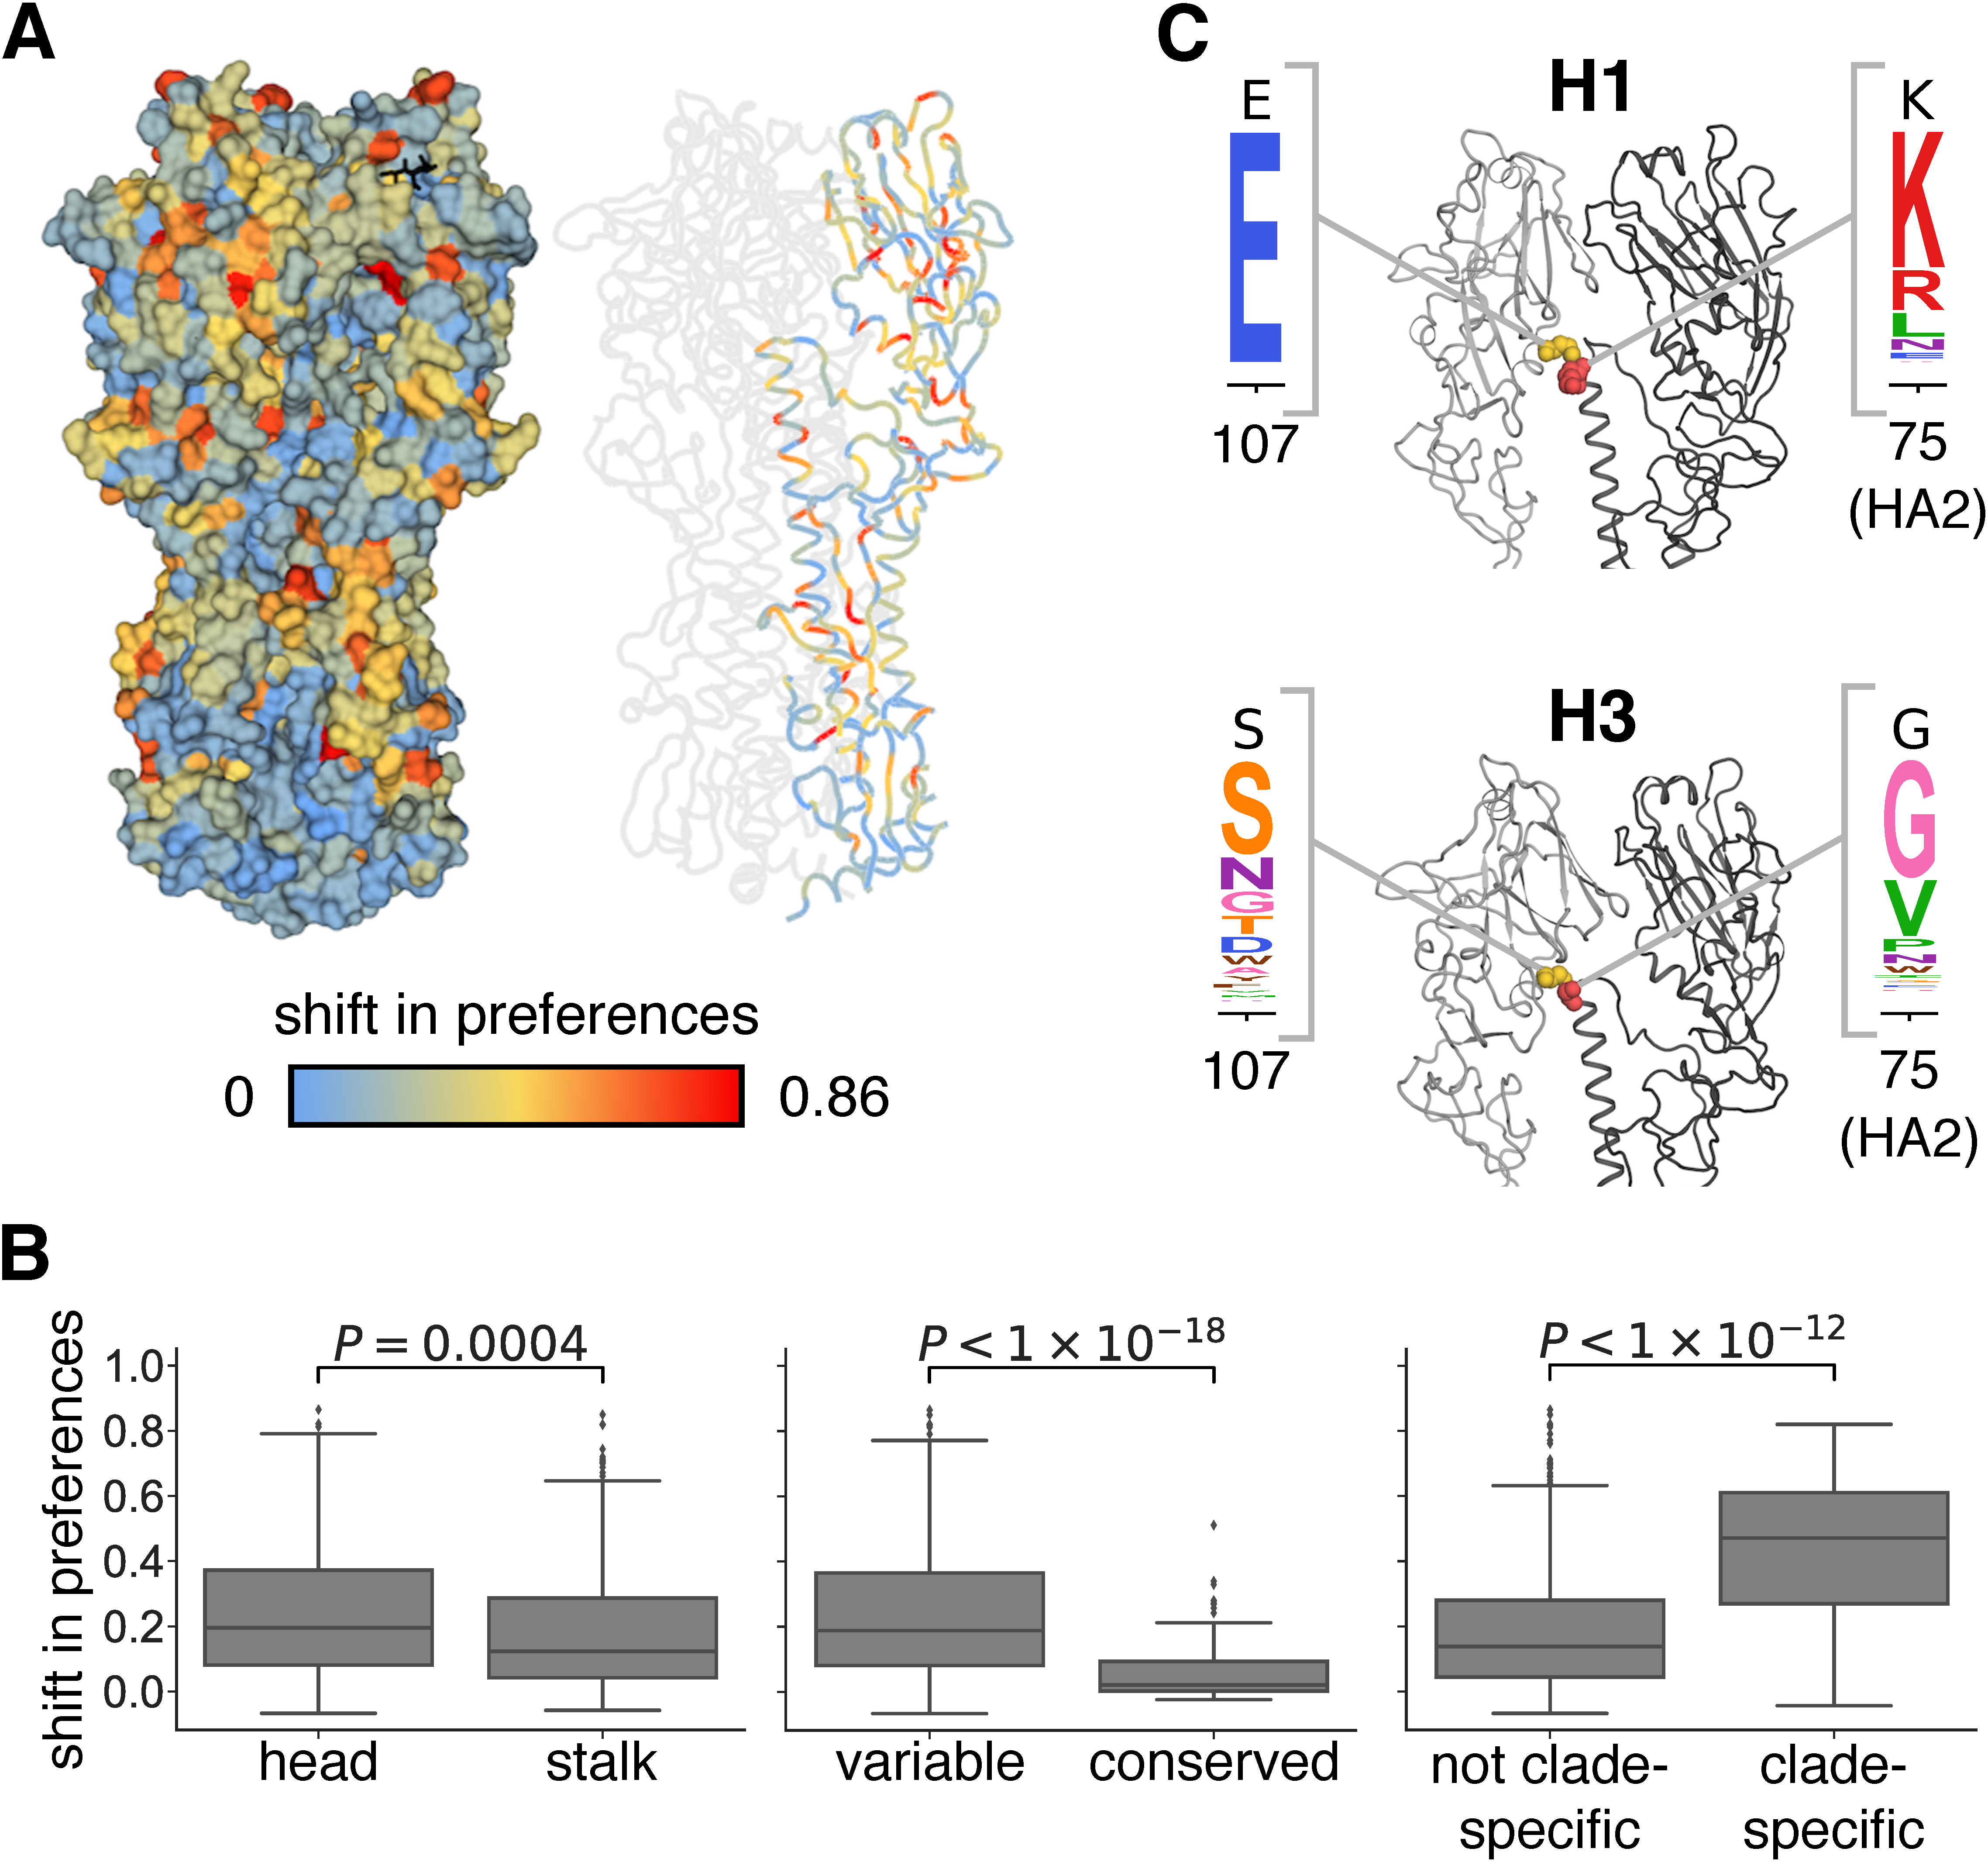
\includegraphics[width=17cm]{figs/RMSD_heatmap/RMSD_heatmap.pdf}
\caption{\label{fig:RMSD_heatmap}
{\bf Characterization of the preference shifts}
(A) The preference shifts as calculated by $\textit{RMSD}_\textit{corrected}$ between the two HA homologs is mapped onto the structure of HA (PDB 4O5N;~\cite{lee2014receptor}). 
The left structure shows the HA trimer, and the right structure colors one of the monomers. 
The sialic acid receptor is shown in black sticks.
Blue indicates small shifts in preference near zero, while red indicates large shifts in preference.
(B) The stalk domain was found to be significantly less shifted than the head domain (left plot).
Sites absolutely conserved all 18 HA subtypes were also found to be significantly less shifted than the remaining non-conserved sites (middle plot).
Sites specific to the clade containing H1, H2, H5, and H6 and specific to the H3, H4, and H14 clade are significantly more shifted than non-clade-specific sites (right plot).
(C) HA group-specific interactions between sites 107 and 75(HA2) play a role in determining the upward translation of the globular head domain relative to the stalk domain.
The amino acids at sites 107 and 75(HA2) are shown in spheres on the structure of H1 and H3. 
One monomer is shown in dark gray, while the HA1 domain of the neighboring monomer is in lighter gray.
The sphere colors correspond to the shift in preference at that site.
The preferences for each site in WSN/1933 and Perth/2009 are also shown.
}
\end{figure*}

\section*{Discussion}
\label{sec:discussion}
We have measured the effect of all possible single amino-acid mutations to Perth/2009 H3 on viral growth in cell culture.

\matmethods{Please describe your materials and methods here. This can be more than one paragraph, and may contain subsections and equations as required. Authors should include a statement in the methods section describing how readers will be able to access the data in the paper.

\subsection*{HA numbering}
Unless otherwise indicated, all sites are in H3 numbering, with the signal peptide in negative numbers, the HA1 subunit in plain numbers, and the HA2 subunit denoted with "(HA2)". The conversion between sequential numbering of the A/Perth/16/2009 HA and H3 numbering was performed using an HA numbering Python script (available at \url{https://github.com/jbloomlab/HA_numbering}).

\subsection*{Creation of MDCK-SIAT1-TMPRSS2 cell line}
The human TMPRSS2 cDNA ORF was ordered from OriGene (NM\_005656), PCR amplified, and cloned into a pHAGE2 lentiviral vector under an EF1$\alpha$-Int promoter and attached to mCherry through an IRES...etc etc
\comment{Need to look at Katie's notebooks for this...}

\subsection*{Generation of HA codon mutant plasmid libraries}
Recombinant A/Perth/16/2009 (HA, NA) $\times$ A/Puerto Rico/8/1934 influenza virus, NIB-64, NR-41803 was ordered from BEI Resources, NIAID, NIH. 
Bulk RNA from the viral sample was extracted using the QIAamp Viral RNA Mini Kit (QIAGEN) according to manufacturer's instructions.
The Perth/2009 HA and NA genes were then reverse transcribed, PCR amplified, and cloned into the pHW2000~\citep{hoffmann2000dna} and pICR2 \comment{cite?} plasmid backbones.

The codon-mutant libraries were generated using a PCR-based approach described in~\cite{bloom2014experimentally,dingens2017comprehensive}.

\subsection*{Generation and passaging of mutant viruses}
The mutant virus libraries were generated and passaged using the approach described in~\cite{doud2016accurate} with several modifications.

\subsection*{Barcoded subamplicon sequencing}

\subsection*{Analysis of deep sequencing data}

\subsection*{Inference of phylogenetic trees}
\comment{We downloaded X sequences from the Influenza Virus Resource ?.... etc. inferred the tree, ancestral state reconstruction, visualized the tree...}
To parse out trunk mutations from side branch mutations, we first defined a set of recent nodes sampled on or after Jan. 1, 2017, and traced these nodes back to their most recent common ancestor. 

\subsection*{Quantification of mutational effects and sequence preferences from an H3N2 phylogeny}

\subsection*{Data availability and source code}
Deep sequencing data are available from the Sequence Read Archive under BioSample accessions SAMN08102609 and SAMN08102610. Computer code used to analyze the data and produce the results in the paper are in...
}

\showmatmethods{} % Display the Materials and Methods section

\acknow{We thank Sarah Hilton, Hugh Haddox, Sidney Bell...the Fred Hutch Genomics Core...
Funding...}

\showacknow{} % Display the acknowledgments section

% \pnasbreak splits and balances the columns before the references.
% Uncomment \pnasbreak to view the references in the PNAS-style
% If you see unexpected formatting errors, try commenting out \pnasbreak
% as it can run into problems with floats and footnotes on the final page.
%\pnasbreak

% Bibliography
\subsection*{References}
\bibliography{references}

% Supplementary material temporarily moved until AFTER everything else for initial submission

\onecolumn

\subsection*{Supporting Information (SI)}
\FloatBarrier

The main text of the paper must stand on its own without the SI. Refer to SI in the manuscript at an appropriate point in the text. Number supporting figures and tables starting with S1, S2, etc. Authors are limited to no more than 10 SI files, not including movie files. Authors who place detailed materials and methods in SI must provide sufficient detail in the main text methods to enable a reader to follow the logic of the procedures and results and also must reference the online methods. If a paper is fundamentally a study of a new method or technique, then the methods must be described completely in the main text. Because PNAS edits SI and composes it into a single PDF, authors must provide the following file formats only.

\subsubsection*{SI Text}

Supply Word, RTF, or LaTeX files (LaTeX files must be accompanied by a PDF with the same file name for visual reference).

\subsubsection*{SI Figures}

\begin{suppfigure}
\centerline{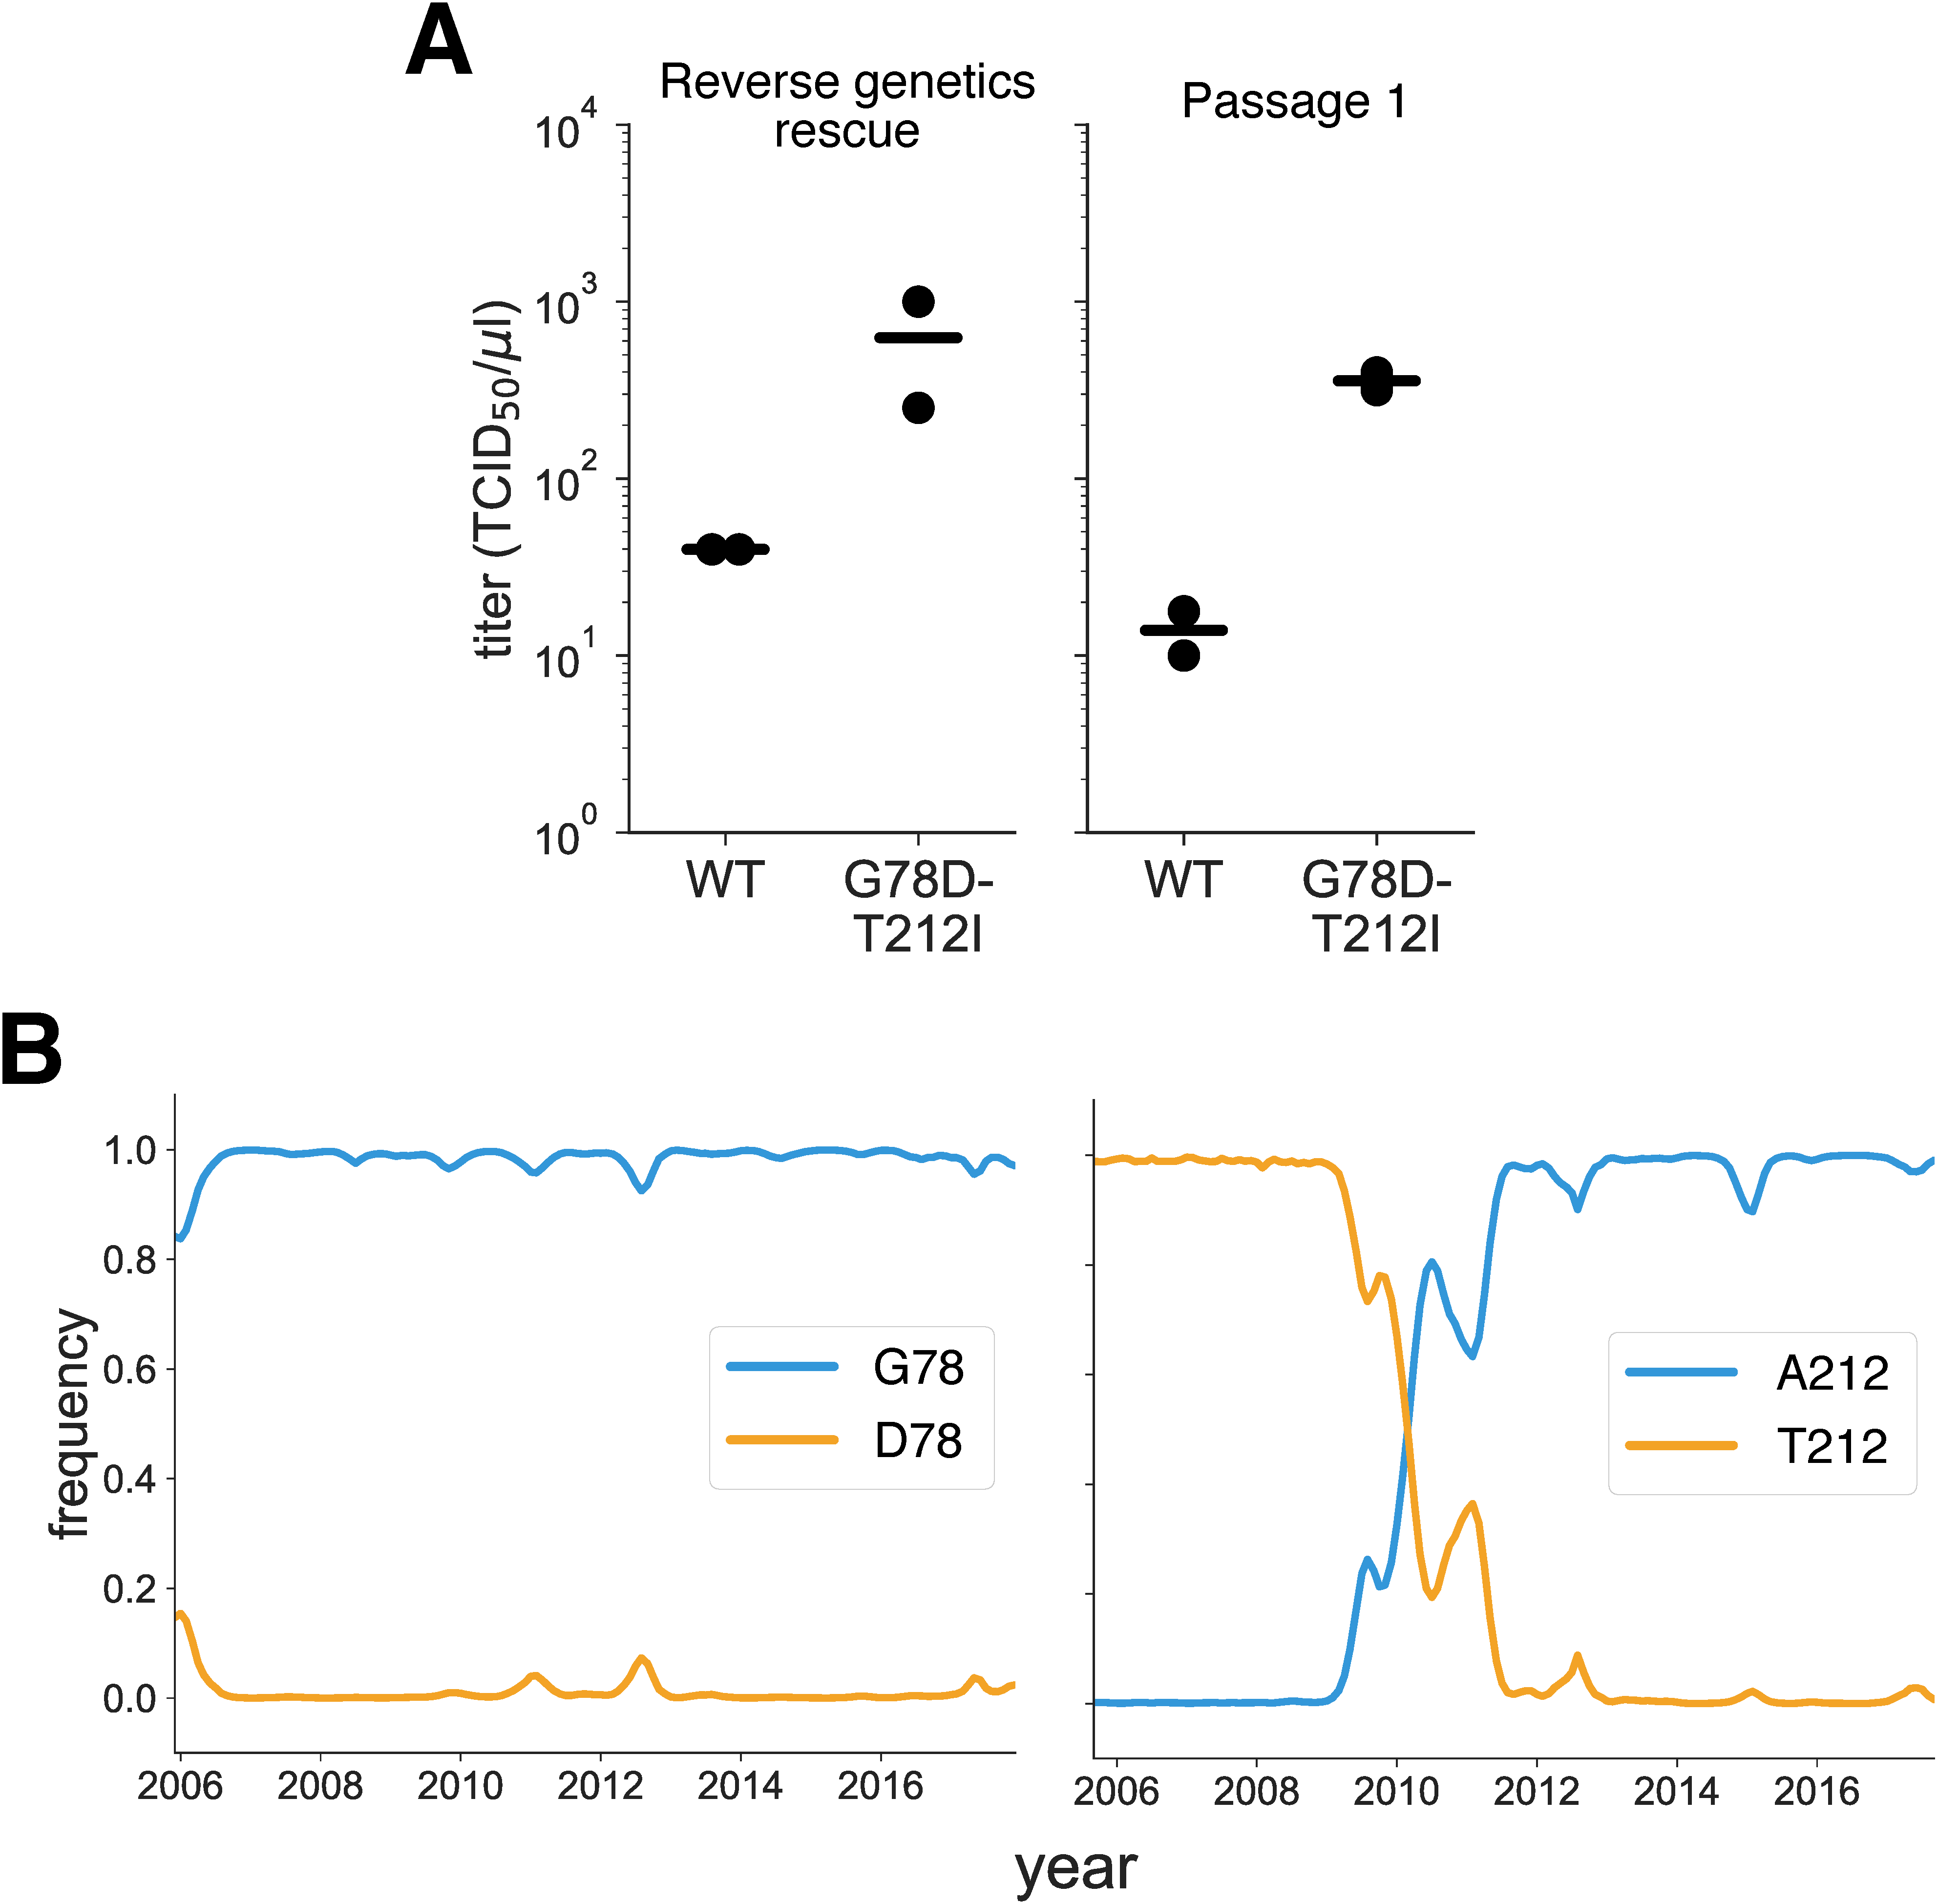
\includegraphics[width=0.5\textwidth]{figs/S01_G78D-T212I/G78D-T212I.pdf}}
\caption{\label{suppfig:Perth2009_mut}
{\bf Characterization of the G78D-T212I Perth/2009 HA variant.} 
(A) 
The G78D-T212I Perth/2009 HA variant supports better viral growth than the wildtype Perth/2009 HA.
Viruses were generated in duplicate by reverse genetics with the Perth/2009 NA and WSN internal genes, and passaged once at MOI = 0.01 in MDCK-SIAT1-TMPRSS2 cells.
The rescue and passage viral supernatants were collected at 72 hours post-transfection and 44 hours post-infection, respectively, and titered in MDCK-SIAT1-TMPRSS2 cells. 
The points mark each duplicate and the bar marks the mean.
(B)
The D78 variant remained at a low frequency in natural human H3N2 sequences over the past $~\sim$10 years.
The A212 variant rose to fixation in $~\sim$2011, replacing the T212 variant.
}
\end{suppfigure}

\begin{suppfigure}
\centerline{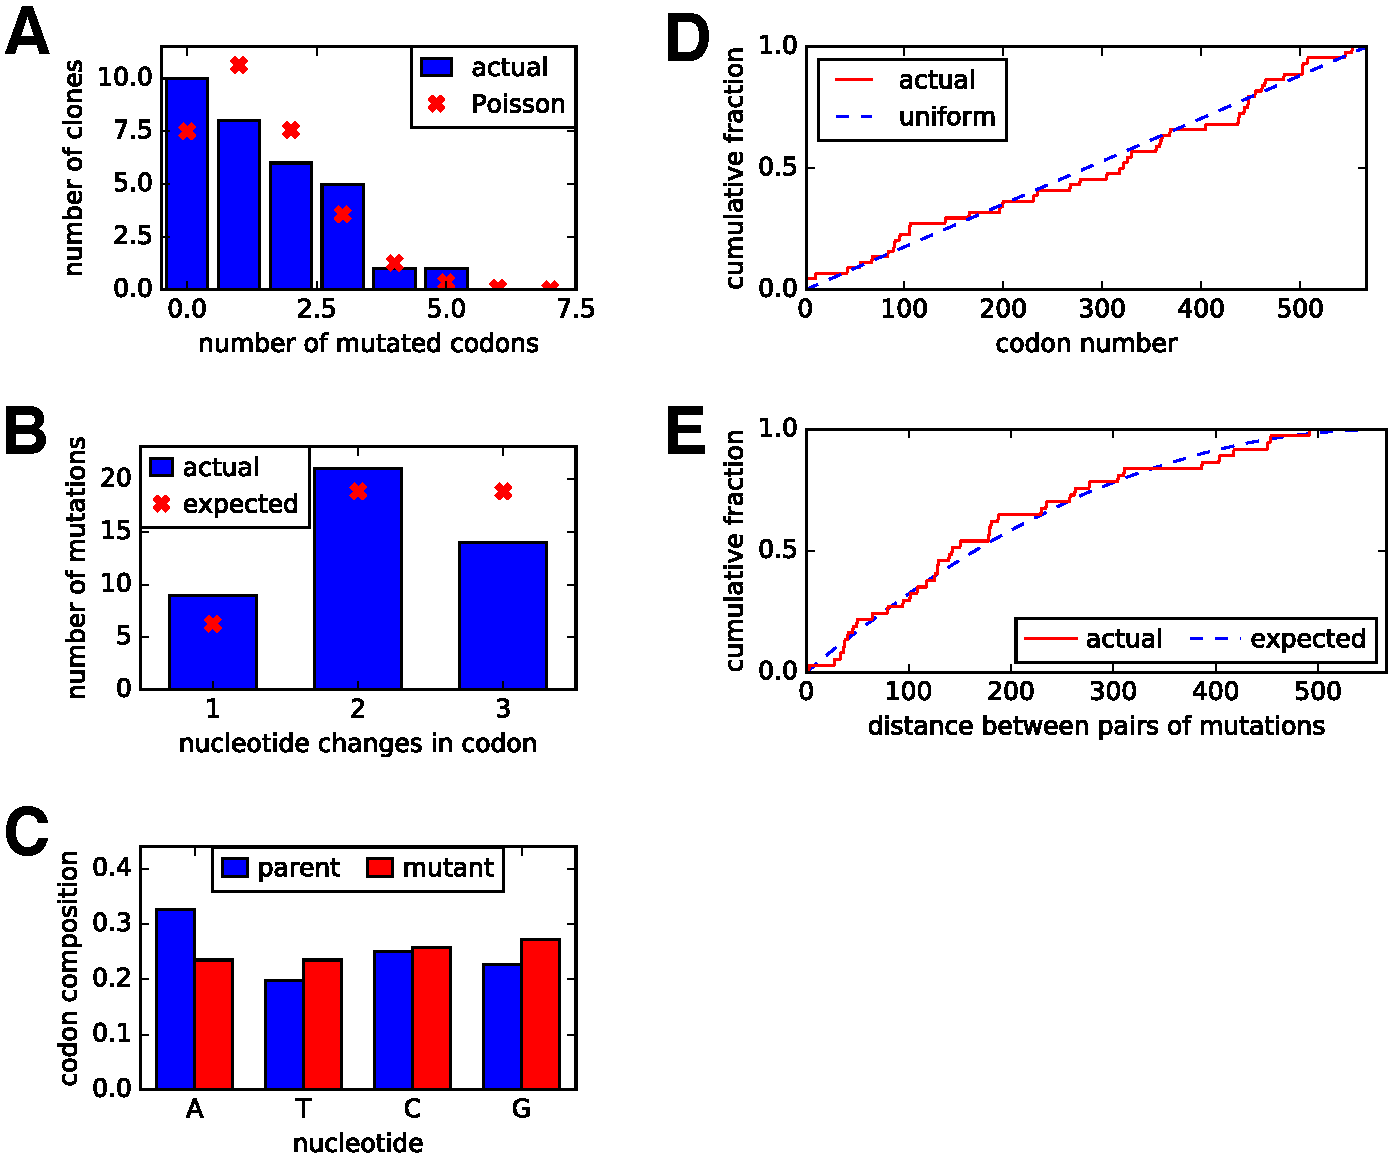
\includegraphics[width=0.6\textwidth]{figs/S02_SangerSeq/SangerSeq.pdf}}
\caption{\label{suppfig:SangerSeq}
{\bf Sanger sequencing of 31 clones from the mutant plasmid libraries.} 
(A) There were an average of $\sim$1.4 codon mutations per clone across the three plasmid mutant libraries.
(B) A mixture of one-, two-, and three-nucleotide mutations were present, with slightly fewer triple-nucleotide changes than expected.
(C) Nucleotide frequencies were uniform in the codon mutations.
(D) The mutations were distributed relatively evenly across the length of the HA coding sequence.
(E) We calculated the pairwise distances between mutations for clones carrying more than one mutation.
The cumulative distribution of the distances is shown in the red line.  
}
\end{suppfigure}

\begin{suppfigure}
\centerline{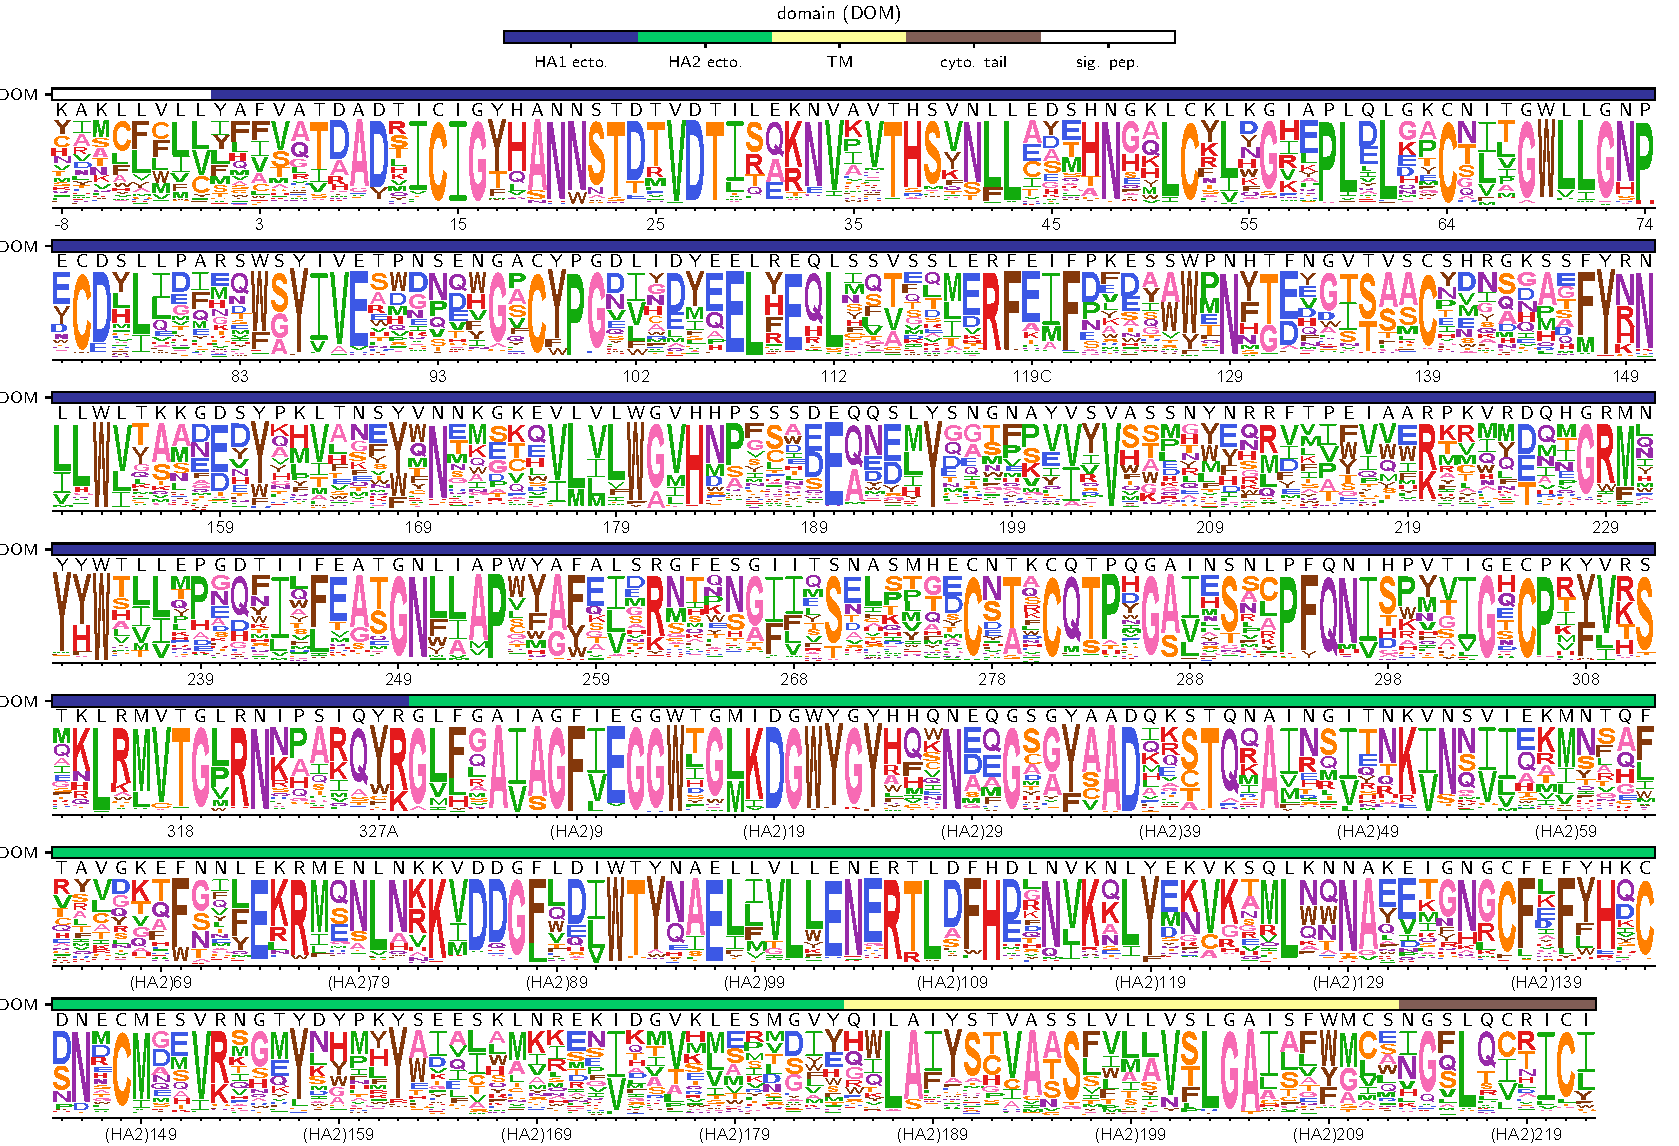
\includegraphics[width=\textwidth]{figs/S03_WSNprefs_logoplot/WSN-rescaled_prefs.pdf}}
\caption{\label{suppfig:WSNprefs_logoplot}
{\bf The site-specific amino-acid preferences of the WSN/1933 H1 HA.} 
}
\end{suppfigure}

\subsubsection*{SI Tables}

Supply Word, RTF, or LaTeX files (LaTeX files must be accompanied by a PDF with the same file name for visual reference); include only one table per file. Do not use tabs or spaces to separate columns in Word tables.

\subsubsection*{SI Datasets} 

\begin{suppdata}
\caption{\label{suppdata:PerthHA}
Genbank file giving the full sequence of the bidirectional reverse-genetics plasmid pHW-Perth2009-HA-G78D-T212I, which encodes the wildtype HA sequence used in this study.
}
\end{suppdata}


\end{document}